%%
%% This is file `example.tex',
%% generated with the docstrip utility.
%%
%% The original source files were:
%%
%% coppe.dtx  (with options: `example')
%% 
%% This is a sample monograph which illustrates the use of `coppe' document
%% class and `coppe-unsrt' BibTeX style.
%% 
%% \CheckSum{1613}
%% \CharacterTable
%%  {Upper-case    \A\B\C\D\E\F\G\H\I\J\K\L\M\N\O\P\Q\R\S\T\U\V\W\X\Y\Z
%%   Lower-case    \a\b\c\d\e\f\g\h\i\j\k\l\m\n\o\p\q\r\s\t\u\v\w\x\y\z
%%   Digits        \0\1\2\3\4\5\6\7\8\9
%%   Exclamation   \!     Double quote  \"     Hash (number) \#
%%   Dollar        \$     Percent       \%     Ampersand     \&
%%   Acute accent  \'     Left paren    \(     Right paren   \)
%%   Asterisk      \*     Plus          \+     Comma         \,
%%   Minus         \-     Point         \.     Solidus       \/
%%   Colon         \:     Semicolon     \;     Less than     \<
%%   Equals        \=     Greater than  \>     Question mark \?
%%   Commercial at \@     Left bracket  \[     Backslash     \\
%%   Right bracket \]     Circumflex    \^     Underscore    \_
%%   Grave accent  \`     Left brace    \{     Vertical bar  \|
%%   Right brace   \}     Tilde         \~}
%%
\documentclass[dsc,numbers]{coppe}
\usepackage{amsmath,amssymb}
\usepackage{hyperref}

% circuitos e tikz
\usepackage{tikz, tkz-euclide} 
\usepackage[europeanresistors,americaninductors]{circuitikz}
\usetikzlibrary{chains}
\usepackage{siunitx}
\usepackage{tikz-qtree}

\usepackage{pgfplots}

\pgfplotsset{compat=1.18}
%

\makelosymbols
\makeloabbreviations
\usepackage[dvipsnames]{xcolor} % letras coloridas

\begin{document}
  \title{T\'itulo da Tese}
  \foreigntitle{Thesis Title}
  \author{Nome do Autor}{Sobrenome}
  \advisor{Prof.}{Nome do Primeiro Orientador}{Sobrenome}{D.Sc.}
  \advisor{Prof.}{Nome do Segundo Orientador}{Sobrenome}{Ph.D.}
  \advisor{Prof.}{Nome do Terceiro Orientador}{Sobrenome}{D.Sc.}

  \examiner{Prof.}{Nome do Primeiro Examinador Sobrenome}{D.Sc.}
  \examiner{Prof.}{Nome do Segundo Examinador Sobrenome}{Ph.D.}
  \examiner{Prof.}{Nome do Terceiro Examinador Sobrenome}{D.Sc.}
  \examiner{Prof.}{Nome do Quarto Examinador Sobrenome}{Ph.D.}
  \examiner{Prof.}{Nome do Quinto Examinador Sobrenome}{Ph.D.}
  \department{PEC}
  \date{05}{2022}

  \keyword{Primeira palavra-chave}
  \keyword{Segunda palavra-chave}
  \keyword{Terceira palavra-chave}

  \maketitle

  \frontmatter
  \dedication{A algu\'em cujo valor \'e digno desta dedicat\'oria.}

  \chapter*{Agradecimentos}

  Gostaria de agradecer a todos.

  \begin{abstract}

  Apresenta-se, nesta tese, ...

  \end{abstract}

  \begin{foreignabstract}

  In this work, we present ...

  \end{foreignabstract}

  \tableofcontents
  \listoffigures
  \listoftables
  \printlosymbols
  \printloabbreviations

  \mainmatter
%%%%%%%%%%%%%%%%%%%%%%%%%%%%%%%%%%%%%%%%%%%%%%%%%%%%%%%%%%  
% Summary.
%1. Introduction
%  1.1 The Motor Drive System
%    1.1.1 The Basic Protection Schemes
%  1.2 Organization of the Dissertation

%2. Literature Review
%  2.1 Reliability Engineering and Power Electronics
%    2.1.1 Physical Analytics
%    2.1.2 Design and Verification
%    2.1.3 Control and Monitoring
%          (The Role of the Protection.)
%  2.2 Fault Detection and Diagnosis
%    2.2.1 Principal Fault Mechanisms at the inverter
%    2.2.2 Fault Consequences for the Inverter and              the motor.
%    2.2.2 A Review on the Principal Fault Detection 
%             Strategies
%      2.2.2.1 DC Offset Based Methods
%      2.2.2.2 Voltage Based Methods
%      2.2.2.3 Spectrum Analysis and Wavelet Based  
%                  Methods
%  2.3 Remaining Useful Life and Prognosis.
%  2.4 Summary

%3. Methodology

%4. Results and Analysis

%5. Further Research

\chapter{Introduction}

The Power Electronics (PE) technology has been evolving in the last five decades with applications spread through the industrial, commercial and residential environment. This diffusion is due to the reduction of cost, size and improvement of performance. Among these applications, there are systems with special requirements to guarantee that the final product has higher standards of safety and availability. One of those concerns is reliability.  This work aims to study the ways to add reliability to one of the PE devices, the inverter,  through condition monitoring using the commonly available signals, like the output currents and voltages. 

One of the tasks of the PE is to process and control the flow of energy and another is to supply the optimal currents and voltages to the load. The nature of this task demands lower energy losses as much as possible due to both the energy costs and the difficulty of removing the heat produced by the losses. These demands have been fulfilled by the advances in semiconductor devices that can be operated intermittently. This activity reproduces patterns of currents and voltages by opening and closing at high frequencies. This results in an operation with inferior ohmic losses than the common electronics topologies.

The power converter is a device with PE to manage energetic trades in many systems.  In the utility grid, they are applied in alternate current (AC) and direct current (DC) power supplies; Electrochemical processes like electrolysis and electroplating, just to name a few. In fact, in a modern industrial environment, PE works closely with computers to support motion control giving high industrial productivity with improved product quality.

\begin{figure}
    \centering
    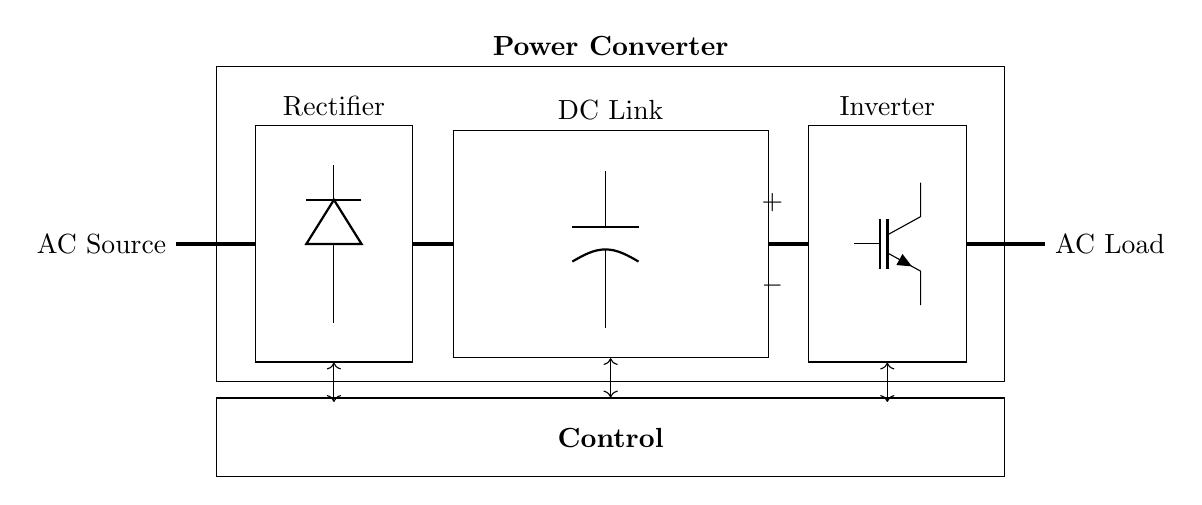
\begin{tikzpicture}[
	start chain = going right,
	box/.style = {
		on chain,join,draw,
		minimum height = 3cm,
		text centered,
		minimum width = 2cm,
	},
	every join/.style={ultra thick},
	node distance=5mm
]

\node [on chain] {AC Source}; % Chain starts here
\node [box, xshift=5mm, label = above: Rectifier] (rec) {
	\begin{circuitikz}
		\draw (0,0) to[Do] (0,2);
	\end{circuitikz}
};

\node [on chain, join, draw, 
	text width=1cm,
	minimum width=4cm,
	minimum height=1.6cm,
	label=above:DC Link,
] (ic) {
    \begin{circuitikz}[american voltages]
		\draw (0,0) to[pC, v<= $ $] (0,2);
	\end{circuitikz}
};

\node [box,label = above:Inverter] (inv) {
	\begin{circuitikz}
		\draw (0,0) node[nigbt] {};
	\end{circuitikz}
};

\node [on chain, join, xshift=5mm]{AC Load};
% Chain ends here

% CU box
\node [
	rectangle,draw,
	below=5mm of ic,
	minimum width=10cm,
	minimum height=1cm,
] (cu) {\textbf{Control}};

% PU box
\node [
	rectangle,draw,
	above=2mm of cu,
	minimum width=10cm,
	minimum height=4cm,
	label=\textbf{Power Converter},
] (pu) {};

% Connections between CU and PU
\draw[<->] (rec.south) -- ++(0,-5mm);
\draw[<->] (cu.north) to (ic.south);
\draw[<->] (inv.south) -- ++(0,-5mm);

\end{tikzpicture}
    \caption{Diagram of the converter main parts.}
    \label{fig:blocosdoconversor}
\end{figure}

The association with motors for activation and control in systems is called motor drives. The motor drives area includes transportation, home appliances, pumps, compressors, wind generation systems... In figure \ref{fig:blocosdoconversor}, a simple converter can be seen with three basic parts to connect the device to the utility grid: the rectifier, the direct-current (DC) link and the inverter (figure one). The rectifier transforms AC signals into DC. The DC link has filters to establish current or voltages between levels to feed the inverter, which in turn transforms the DC signal back to AC, according to the needs of the load. 

Such systems have different demands according to where it's applied. For example, a pump that works two hours a day has different needs than an electric vehicle motor drive. Critical applications are those with special needs, like higher availability, reliability, robustness or low failure rate. The usual engineering definitions of these concepts are listed as follows to be used in this work \cite{Patrick2011_2}:
 \begin{itemize}
     \item Reliability is the ability of a system to function under desired conditions within a specific period. Its frequently expressed in failures per period;
     \item Durability, a particular aspect of reliability, is to withstand the effects of time. It can be fatigue, wear, electrical parameter change, and so on. It can be expressed as the minimum time before wear.  
     \item Robustness, though, can be defined as the degree to which a system can function correctly in the presence of inputs different from those assumed. In a more general sense, a robust system can endure a wide range of operating conditions \cite{AliMaciejewski04}.
     \item Maintainability is the ease with which repairs and other maintenance work can be carried out \cite{Patrick2011_3}. 
\end{itemize}

Maintainability affects the availability of the system directly. The repair routines usually remove the system from the available state. Thus, easier maintainability implies shorter repair stops and higher availability. Also, there is higher availability when the distance between maintenance events is larger. In this case, it is related to reliability. In \cite{Patrick2011_3}, maintainability is said to be closely related to reliability as they impact final costs. 

A device suitable to work with a wind turbine, for example, has high availability requirements to perform its tasks. That's because maintenance, and specially non-planned maintenance, is costly. In this case, the maintenance stops prevent the energy generation which increases the energy total costs that pass on to the customers.

To illustrate these terms in a critical system such as the wind energy industry, the work \cite{CEVASCO2021} reviews data on some of the principal wind farms. The data on the availability of onshore wind turbines have been shown to reach values in a range of 95–97\% for modern systems. For offshore projects, however, the location and challenges, like accessibility and harsh weather conditions, can lower availability. As commented by the authors, older farms – comprising turbines with relatively low nominal capacity, and closer to the coast – exhibit an availability in the range of the onshore average one. Newer farms – bigger and located further from the coast – are characterized by an increase in maintenance efforts.

\cite{Pfaffel2017} developed a detailed analysis at the subsystem level for wind turbines with the WMEP (Wissenschaftliches Mess-und Evaluierungsprogramm), a German database. This research is also reviewed in \cite{CEVASCO2021}. The authors found differences in the contribution of single components’ failures to the total failure frequency for small and large-sized turbines. A smaller scatter for the share of each system to the failure rate is generally observed for medium rating turbines (above 500 kW and below 1.5 MW), whereas the reduction in the percentage failure of the mechanical and structural components is balanced by an increase in the percentage of the electrical failures for the high power class. 

Figure \ref{fig:WTfailure} reproduces the resultant plot of power rating per share to the failure rate from the work of \cite{CEVASCO2021}. The control system is labeled as box-plot 5 and presents the minimum failure rate near 15\% for the category of 0 to 30 kW and the maximum near 20\% for the 1000 to 1500 kW. The group of transmission, converter, generator and transformer systems is labeled as box-plot 7 and has a minimum between 15-20\% for the 0-30 kW category and a maximum near 35\% for the above 1500 kW rating.  It's interesting to see that a high power rating registered a lower failure rate for the control systems than the middle rating of 1000-15000 kW.  As these two groups, electrical and control systems, are associated with the overall rise of the annual failure frequency, they can be seen as the most critical components for the WMEP larger-sized turbines.

\begin{figure}
    \centering
    \includegraphics{figuras/Total average failure rate of wind turbines of each group of MW-class.jpg}
    \caption{graph of the total average failure rate of subsystems in wind turbines.}
    \label{fig:WTfailure}
\end{figure}

Other industries convey similar concerns with PE reliability. In \cite{ShaoyongY2011}, a survey with agents of the automotive, aerospatial, component manufacturer, utility and motor drive sectors was made in 2009. According to those agents, the IGBTs, capacitors and gate drivers are said to be the most fragile components of the system in that order. The maintenance stops are most related to transients of the system, followed by overload and environmental effects. The increase in temperature is cited as the most serious environmental factor that is a precursor to failure. 

The survey also shares how each sector handles the reliability problems in their applications. The component manufacturers highlight the voltage suppressors while the aerospatial sector and the utility, the back-ups. The automotive and motor drives, in turn, are fond of the increase in the coolant. Figure three represents a heat map with the number of answers of the sectors and their respective item. The authors emphasized that high-duty cycle applications, like 365 days a year in the utility grid, are likely to prefer back-ups due to avoid maintenance stops.

\begin{figure}
    \centering
    \includegraphics{figuras/correlacaoconfiabilidadesetores.png}
    \caption{Caption}
    \label{fig:my_label}
\end{figure}
Figure three: survey correlation map.

Another approach to handling reliability issues is to anticipate the failure as much as possible so that the operation of the system can be halted before a breakdown occurs. During these stops, preventive maintenance is arranged to retain the system in the available state. This means substituting damaged parts, cleaning, lubricating and inspections to counter improper behavior or incipient faults.

To increase the efficiency of the scheduled maintenance, information with valuable features must be collected. In \cite{Yang2010}, the monitoring of a system is classified into three categories: 
Diagnosis: Identifying the root cause of failure;
Prognosis: Predicting the state of the component in the future;   
Condition Monitoring (CM): Real-time measurement of a component or a system and taking appropriate actions. 
Figure \ref{fig:complete_heath_monitoring} presents a version of a complete condition monitoring system for a power converter. The sensors gather data on important parameters for converters like output current, voltages and temperatures. The data is processed to extract damage indicators that can be read by the CM unit. If there is an incipient fault condition, the diagnosis unit sends a message to change the control of the converter to operate in a degraded mode until the maintenance time. The prognosis unit, in turn, process the indicators to determine the time for the maintenance. If a fault condition is found, changes can be done in the control to avoid a catastrophic failure or a complete halt of the system. 

\begin{figure}
    \centering
    \includegraphics{figuras/complete health-monitoring system.jpg}
    \caption{Scheme of a complete monitoring system.}
    \label{fig:complete_heath_monitoring}
\end{figure}

Bearing in mind the importance of PE supporting critical applications, this work aims to study the main condition monitoring strategies for a power inverter. Especially those concerned with the IGBT condition, because is considered to be one of the fragile components of this system. Among the divisions in this field, software-dependent techniques are preferred, instead of hardware-dependent ones. Hence, a review of the recent works is presented in chapter  2. Once the main strategies are discussed, chapter 3 presents a methodology to apply the suitable ones in the data extracted from a simulated motor drive system.  Chapter 4 shows the results and performance analysis while Chapter 5 presents a conclusion and further work.

\section{The Motor Drive System}
\subsection{The Basic Protection Schemes}
%\section{How the Dissertation is Organized.}
\chapter{Literature Review}

\section{Reliability Engineering and Power Electronics}
Historically, the perception of Reliability Engineering (RE) as a discipline was possible through the development of statistics and mass production \cite{SALEH2006249}. In essence, reliability engineering is to prevent the creation of failures, especially in the early stages. Because a flaw found in these stages of production, or of design, affects all produced items and the cost to correct them increases progressively as the production proceeds. 
Since the beginning of the XX century, approaches were developed to handle reliability issues in large-scale productions. The branch that dominated the USA until the 1980s was the specification of quantitative reliability requirements. This approach models and collects as much field-failure data as possible, statistically analyzes them, and quantifies model parameters based on the statistical analysis. The failure models and data were published in handbooks, like the [reference], by the defense department of the EUA and industrial groups.

According to the historical review in \cite{Denson98}, the advances in technology and the growth of integrated circuits (IC) presented challenges to the reliability models of the handbooks. In the 1990s, even though new empirical models were crafted to handle the ICs' reliability issues, the ICs devolved into more complex devices and those models received many critics from the user community. Most of them argue that those models were too complex for the user (industry) and unrealistic in the sense that some required data was hardly ever provided by manufacturers because of the competitive strategy.

For these reasons, another approach gained the attention of scientists and engineers: the Physics-Of-Failure (POF). Instead of relying on field-fault data and empirical models, POF is based on the study of physical processes responsible for failures and factors like manufacturing, design, and system requirements. 

In the paper of \cite{HuaiWang2021} and the book chapter of \cite{Chung2015}, a parallel was drawn demonstrating the evolution of power electronics and reliability engineering along the XX century.  The timelines of figure \ref{fig:timeline} divided the century into periods and show selected main issues for each period for both disciplines. A good part of the research in power electronics developed the semiconductor technology, packaging and control strategies we have today. Meanwhile, more and more reliable production processes and devices made it possible to offer those products for a large number of applications. In the later 1990s, the advances in prototyping and simulations allowed projects to attend to the demands of more sophisticated profiles. 

\begin{figure}
    \centering
    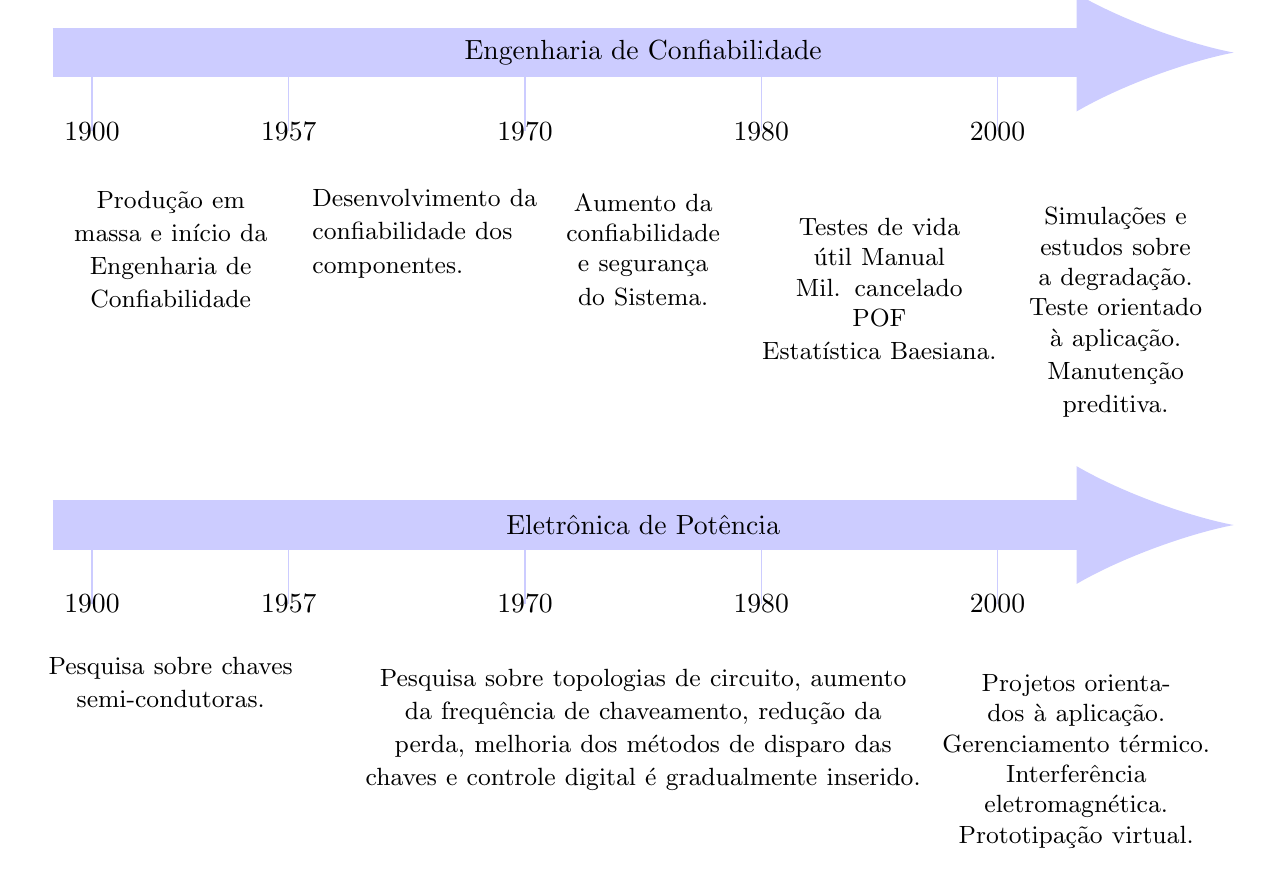
\begin{tikzpicture}
% textos da linha temporal da confiabilidade.
\node [align = center, text width = 3cm](texto1900) at (1.5, -2.5){\small Produção em massa e início da Engenharia de  Confiabilidade};
\node [align = left, text width = 3cm](texto1957) at (4.8, -2.3){ \small Desenvolvimento da confiabilidade dos componentes.};
\node [align = center, text width = 3cm](texto1970) at (7.5, -2.5){\small Aumento da confiabilidade e segurança \\\small do Sistema.};
\node [align = center, text width = 3.2cm](texto1980) at (10.5, -3.){\small Testes de vida útil Manual Mil. cancelado \\ \small POF\\ \small Estatística Baesiana.};
\node [align = center, text width = 3cm](texto2000) at (13.5, -3.3){\small Simulações e \\ \small estudos sobre a degradação. Teste orientado à aplicação.\\ \small Manutenção preditiva.};
%\draw[-{Triangle[width=18pt,length=8pt]}, line width=12pt](0,0) -- (15, 0);
\draw[->, >=latex, blue!20!white, line width=18pt] (0,0) to node[black]{Engenharia de Confiabilidade} (15,0);
\draw [blue!20!white](0.5,0.1) -- (0.5,-1.) node [black]{1900};
\draw [blue!20!white](3,0.1) -- (3,-1.) node [black]{1957};
\draw [blue!20!white](6,0.1) -- (6, -1.) node [black]{1970};
\draw [blue!20!white](9,0.1) -- (9, -1.) node [black]{1980};
\draw [blue!20!white](12,0.1) -- (12, -1) node [black]{2000};

% Textos da linha temporal de eletrônica de potência.
\node [align = center, text width = 3.2cm] at (1.5,-8){\small Pesquisa sobre chaves semi-condutoras.};
\node [align = center, text width = 7.2cm] at (7.5,-8.6){\small Pesquisa sobre topologias de circuito, aumento da frequência de chaveamento, redução da perda, melhoria dos métodos de disparo das chaves e controle digital é gradualmente inserido.};
\node [align = center, text width = 3.6cm] at (13,-9.0){\small Projetos orientados à aplicação. \\ \small Gerenciamento térmico. \\ \small Interferência eletromagnética. \\ \small Prototipação virtual. \\ };
\draw[->, >=latex, blue!20!white, line width=18pt] (0,-6) to node[black]{Eletrônica de Potência} (15,-6);
\draw [blue!20!white](0.5,-6.1) -- (0.5,-7.) node [black]{1900};
\draw [blue!20!white](3,-6.1) -- (3,-7.) node [black]{1957};
\draw [blue!20!white](6,-6.1) -- (6, -7.) node [black]{1970};
\draw [blue!20!white](9,-6.1) -- (9, -7.) node [black]{1980};
\draw [blue!20!white](12,-6.1) -- (12, -7) node [black]{2000};

\end{tikzpicture}

    \caption{timeline of reliability engineering and power electronics of \cite{HuaiWang2021} e \cite{Chung2015} (adapted).}
    \label{fig:timeline}
\end{figure}

In the work \cite{HuaiWang2021}, the authors argue that reliability engineering in PE devices is of interest to many industries, like the automotive [reference]. However, the approaches presented in works like [reference] reveal that conventional handbook methods are still dominantly applied nowadays for the reliability prediction in PE. One of the reasons for the lack of adoption of the POF is that technology and science are still highly evolving. Many of the POF that works for microelectronics, for example, do not work for PE applications because the thermal stresses and the interaction of components are different.

According to \cite{HuaiWang2021} and [book], the future of PE reliability research can be divided into three parts: the first is analytical physics, which involves a POF approach to understanding why and how devices fail; the second, design for reliability (DFR) and robustness validation process to build in reliability and sufficient robustness in the products during each development process; The last, intelligent control and condition monitoring to ensure reliable field operation under specific mission profiles. Figure \ref{fig:PEreliability} illustrates those subjects with a tree diagram.

\begin{figure}
    \centering
    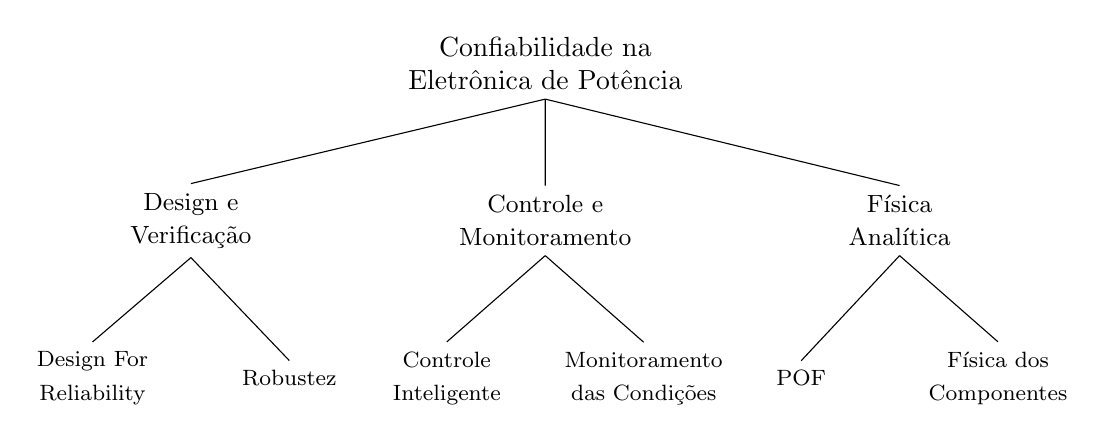
\begin{tikzpicture}
[
    level 1/.style = { sibling distance = 4.5cm},
    level 2/.style = { sibling distance = 2.5cm}
]
 
\node[align = center] {\normalsize Confiabilidade na\\\normalsize Eletrônica de Potência}[sibling distance = 2.cm, level distance = 2cm] 
    child [align = center]{node {\small Design e \\\small Verificação} child {node {\footnotesize Design For\\ \footnotesize Reliability}} 
    child {node {\footnotesize Robustez}}}
    child [align = center]{node {\small Controle e\\\small Monitoramento} child {node {\footnotesize Controle \\\footnotesize Inteligente}}
    child {node {\footnotesize Monitoramento \\\footnotesize das Condições}}}
    child [align = center]{node {\small Física\\\small Analítica}
    child {node {\footnotesize POF}}
    child {node {\footnotesize Física dos\\\footnotesize Componentes}}};
\end{tikzpicture}
    \caption{ Three major parts of the future of PE reliability research according to \cite{HuaiWang2021}.}
    \label{fig:PEreliability}
\end{figure}

This works deals with the condition monitoring related to the converter. The following sections review some of the main works in this area to monitor this device using the commonly available signals.
% Insert review papers of the other areas once it is not covered in this work.

\section{Condition Monitoring}
Condition monitoring (CM), as defined in \cite{Yang2010}, is a technique for monitoring the characteristic of a physical system. Normally, the engineer chooses a set of signals with meaningful features to measure the device's condition. When the extracted features show that the device is drifting away from normal operation, a warning state rise, and corrective actions can be taken. Generally, the role of such systems is to answer if the device will survive until the next maintenance period. 

\begin{figure}
    \centering
    \includegraphics{figuras/complete health-monitoring system.jpg}
    \caption{Complete condition monitoring system.}
    \label{fig:health-monitoring-system}
\end{figure}

In \cite{Yang2010}, the authors share their view on a complete condition monitoring system, detailed in figure \ref{fig:health-monitoring-system}, and two other concepts: prognosis and diagnosis. In the schematic, the sensors have the role of getting data from the power converter and transmitting it to be processed; CM acts to extract features from the raw signals in real-time to feed other parts of the system; The diagnosis uses these features to identify faulty patterns, whereas the prognosis foresees the device's conditions in the future. 

In \cite{Hyunseok2015}, the authors comment on three challenges for condition monitoring: 
1) how to measure physical quantities related to conditions of the device without interrupting their operation; 
2) how to correlate health indicators estimated from physical measurements to the actual conditions of the device; 
3) how to project health indicators to the future with adequate failure criteria and manage uncertainties.

Many studies address these challenges in the power electronics field. Commonly, the semiconductor switches and capacitors are the focus of the monitoring system because of their importance and many field experiences []. One of the switches is the Insulate Gate Bipolar Transistor (IGBT), a highly demanded semiconductor switch for many industries such as wind energy generation. 

The work of \cite{Kastha1994} does investigations on the fault modes of a voltage-fed inverter with mathematical analysis and simulations. The authors aim to use these analyses for the protection system and fault tolerant control. In \cite{Hyunseok2015}, an overview of IGBT modules' technologies and monitoring methods is presented with a discussion of their failure mechanisms and the prognostics techniques. Another review of power electronics monitoring in \cite{Avenas15} divides the techniques into classical and global methods. The classical methods are those which use IGBTs' parameters, like voltages and temperatures, while the global ones use system-level signals, like the output current and voltages.  Solutions with sensors inside the devices to monitor a specific component are said to be classical because they were the first methods documented. For example, the work of [] shows the commonly observed signals for the IGBT.  These parameters are analyzed later in this chapter.

From the point of view of power electronics, the classical strategies in \cite{Avenas15} monitor components with a high-power density trend in the industry which can difficult to detect tiny patterns with sensors inside the device. One example is the VGE signal of the IGBT, shown in figure \ref{fig:VCE-signal}. The signal oscillates between the on and off-state with high frequency and a huge difference in the scale of the measures. Many studies relate an increase in the on-state $V_{CE}$ as the device deteriorates over time []. These experiences require precision hardware to be able to work at this scale. 

\begin{figure}
    \centering
    \includegraphics{figuras/VCE during turn-off.jpg}
    \caption{$V_{CE}$ signal for monitoring.}
    \label{fig:VCE-signal}
\end{figure}


The global strategies commented in \cite{Avenas15} don't need the precision hardware or extra sensors but employ sophisticated signal processing algorithms to extract features. In the work of \cite{BinSantosh09}, the authors review the existing methods for IGBT diagnostics and protection, including open-circuit, short-circuit, and gate-misfiring faults of IGBTs in three-phase power inverters. All the methods use system-level signals such as the inverter's output current. Some of the techniques employ fuzzy, wavelets, and Artificial Intelligence (AI). At the time of the article (2009), the authors consider that these methods render additional intelligence for smart diagnosis at a cost of a higher implementational effort. A question that is of interest for this work is how those methods developed over the years and if they reward a better performance nowadays despite the complexities.

In \cite{Zhao21}, the authors discuss the possibilities of system-level monitoring with AI. This branch has been emerging once the underlying technologies, such as Internet-of-Things (IoT), data storage, and analytics, are evolving fast. Another favorable aspect is that the core of CM is a prediction based on past and present information, which are common tasks that AI can address if there are available data.

However, the authors also point out obstacles to applications in PE systems such as the limited size of the dataset, the heterogeneous operational environment, a limited computational platform, and mission-critical applications. The first issue is that power electronics are not as data-intensive as common AI fields such as image recognition. For example, time-to-failure data is scarce since the degradation process can last for years. Moreover, the computational platform for PE is designed for control and protection purposes. Any other functions can exceed their computation power and bring risks to the system. 

Another concern is that PE is currently employed in a wide range of operational environments, including extreme climatic conditions. These external factors, in turn, can affect
the patterns of the collected data. Aside, most of the demands for CM are also mission-critical which means that the tolerance for false prediction is low. 

In summary, this review covered the concept of CM for PE systems. The research selected articles related to IGBT switches because of their importance to the industry. Then, the research commented on two main sources for CM systems: data from sensors inside the devices or system-level data available for control and protection purposes. This work opts to investigate the strategies with system-level signals once they are prone to cost reduction. Within this branch, applications with all sorts of algorithms can be found and, more recently, AI has emerged as a promising direction. 

The following sections cover topics necessary to understand the algorithms and parameters for monitoring, which are the IGBT's functions, failure mechanisms, known diagnostic algorithms, and how they can track the degradation of the device over time.  Once this subject is discussed, a section for reviewing prominent papers of CM with system-level data is set to inquire about what is the best method for a motor drive system. Then, the rest of this chapter has a discussion and summary of all the works mentioned. 

\section{The IGBT's functions and Failure Mechanisms}
This section discusses the Integrated Gate Bipolar Transistor (IGBT) switches with a view to the condition monitoring of these devices. First, this section presents a review of the switches' technologies and their function, followed by recent works about the known failure mechanisms for the models. 

\subsection{IGBT's Main Technologies}
The semiconductor switch's core functions are performed by the chips, which are stacked semiconductor layers with different levels of impurities. Semiconductors are insulators in a pure state and at room temperature. Because of their valence bonds in the crystalline, there are only a few free electrons due to the thermal energy. Doping is a process that changes a semiconductor's conductivity by adding atoms from other elements to their crystalline structures. Semiconductors such as silicon have more free electrons by adding donor atoms, such as phosphorus, while empty spaces or holes increase by adding trivalent atoms such as boron \cite{malvino2015}.  The semiconductors are of p-type if they are doped to increase the positive charges and of n-type if their negative charges surpass. 

\begin{figure}
    \centering
    \includegraphics{figuras/IGBTbasico.png}
    \caption{Basic IGBT chip}
    \label{fig:IGBTchip}
\end{figure}

The core schematic for an IGBT chip is shown in figure \ref{fig:IGBTchip}. The IGBT has three ports: Gate, Emitter, and Collector. Collector and Emitter are connected with the principal circuit while Gate is connected to Emitter via a secondary circuit.  In this device, a voltage between the Gate-Emitter circuit has the role to control the flow of electrons inside. Therefore, it's a voltage-controlled switch and when a positive voltage is applied between the Gate-Emitter terminals, higher than a bound, an electric field drags the free electrons toward the gate terminals, while the conventional current, the holes, goes to the emitter terminals. However, the electrons never pass through the gates due to an insulating layer between the contact surface.

IGBT chips work encapsulated into modules, as in figure two. While the chip is the source of the basic functions, the exterior package of the module provides electric connections, heat dispersion, and protection against the environment and handling. Many works divide the modules into the die and package. The die is the silicon chip and the exterior package contains all the connections and protections. 

\begin{figure}
    \centering
    \includegraphics{figuras/bondwiremodule.png}
    \caption{The wire-bond module cross-section from \cite{Hyunseok2015}.}
    \label{fig:bondwiremodule}
\end{figure}

According to [Hyunseok2015], there are two kinds of packages for IGBTs widely spread nowadays: The wire-bond and press-pack. Figure \ref{fig:bondwiremodule} shows an example of a cross-section of the wire-bond and figure \ref{fig:ppIGBT}, of the press-pack module. The wire-bond modules are recognized by aluminum wire bonding connections atop the die that link the chips to the output terminals. Visually, a copper base plate serves as an assembly platform for all other components. An inert substance such as silicon gel fills the empty spaces inside the packages to enhance electrical insulation and avoid moisture.  

\begin{figure}
    \centering
    \includegraphics{figuras/presspack.png}
    \caption{The press-pack module cross-section from \cite{Hyunseok2015}.}
    \label{fig:ppIGBT}
\end{figure}


Press-pack modules substitute the wire bond and solder with bondless pressure contacts. Figure \ref{fig:ppIGBT} shows a schematic for one of the market standard models recognized by the cross-section with rigid pillars. The Emitter and Collector terminals (in the pillars) connect to the chip via a molybdenum plate and the Gate is connected to the die through a spring-loaded pin. Without any welding, the thermal and electrical contacts are due to a clamping force from a pressure system that also presses the load terminals \cite{SCHEUERMANN2009}. Figure \ref{fig:ppIGBTexplode} shows an exploded view of the device. In this cylindrical vessel, the components are combined and hermetically closed by a hard-crimping technology. 

\begin{figure}
    \centering
    \includegraphics{figuras/IGBT press-pack3.jpg}
    \caption{An exploded view of the press-pack IGBT from \cite{Hui2019}.}
    \label{fig:ppIGBTexplode}
\end{figure}

Critical concerns for the modules are to guarantee the current path and heat dissipation at the same time. From the perspective of the wire-bond module, the electrical current's path between terminals goes through the aluminum wire, solder joints, copper plates, and the IGBT chip, as shown in figure \ref{fig:bondwiremodule}. Ceramic substrates provide electrical insulation for the device with a help of silicon gel to prevent current arches or sparks inside the module.  

\begin{figure}
    \centering
    \includegraphics{figuras/heat dissipation IGBT.jpg}
    \caption{Heat dissipation path of the wire-bond IGBT from \cite{Narumanchi2008}.}
    \label{fig:IGBTheatpath}
\end{figure}

Figure \ref{fig:IGBTheatpath} from \cite{Narumanchi2008} shows the heat dissipation path for the wire-bond module. The silicon chip transmits the heat to the solder joints, a copper layer, the substrate, the base plate, and finally to the heat sink. The grease layer between the base plate and the heat sink enhances the thermic exchanges between the two parts. 

The electrical path for the press-pack IGBTs is the connections between the lids, molybdenum plate, and the chips. Aside, the press-pack model allows a double heat sink mounted on the Collector and Emitter sides to enhance heat dissipation, an important quality for the transport industry. The next item discusses selected failure modes for the IGBTs in each technology to better understand the advantages and disadvantages of their applications. 

\subsection{Failure Mechanisms}
Texts of reliability engineering such as \cite{Patrick2011_2} explain that failures can happen in a sudden way or by wear-out. Sudden failures are caused by design defects, manufacturing issues, single-event effects, overstress, or misuse. In contrast, wear-out failures are caused by long-term degradation. For a power electronic system, failure can come from both hardware and software due to internal and external factors.  This section grasps only some of the hardware-related failures.

\pgfmathdeclarefunction{gauss}{2}{%
  \pgfmathparse{1/(#2*sqrt(2*pi))*exp(-((x-#1)^2)/(2*#2^2))}%
}
\begin{figure}
    \centering
    
    \begin{tikzpicture}
\begin{axis}[
  no markers, domain=0:20, samples=100,
  axis lines*=left, xlabel=$x$, ylabel=$y$,
  every axis y label/.style={at=(current axis.above origin),anchor=south},
  every axis x label/.style={at=(current axis.right of origin),anchor=west},
  height=3.5cm, width=7.8cm,
  xtick={6,13.5}, ytick=\empty,
  enlargelimits=false, clip=false, axis on top,
  grid = major
  ]
  \addplot [very thick,cyan!50!black] {gauss(6,1)};
  \addplot [very thick,cyan!50!black] {gauss(13.5,1)};

\draw [yshift=-0.8cm, latex-latex](axis cs:10.5,0) -- node [fill=white] {S} (axis cs:16.5,0);
\draw [yshift=-0.8cm, latex-latex](axis cs:3.,0) -- node [fill=white] {L} (axis cs:9,0);

\end{axis}
\begin{axis}[yshift = 2.5cm, xshift = 1.79cm,
  no markers, domain=0:20, samples=100,
  axis lines*=left, xlabel=$x$, ylabel=$y$,
  every axis y label/.style={at=(current axis.above origin),anchor=south},
  every axis x label/.style={at=(current axis.right of origin),anchor=west},
  height=3.5cm, width=7.8cm,
  xtick={6,10.5}, ytick=\empty,
  enlargelimits=false, clip=false, axis on top,
  grid = major
  ]
    \addplot [fill=cyan!20, draw=none, domain=7.5:9] {gauss(6.,1)} \closedcycle;
  \addplot [very thick,cyan!50!black] {gauss(6,1)};
  \addplot [very thick,cyan!50!black] {gauss(10.5,1)};
  \end{axis}
  
  \begin{axis}[yshift = 5.cm, xshift = 3.5cm,
  no markers, domain=0:20, samples=100,
  axis lines*=left, xlabel=$x$, ylabel=$y$,
  every axis y label/.style={at=(current axis.above origin),anchor=south},
  every axis x label/.style={at=(current axis.right of origin),anchor=west},
  height=3.5cm, width=7.8cm,
  xtick={6,9.7}, ytick=\empty,
  enlargelimits=false, clip=false, axis on top,
  grid = major
  ]
  \addplot [fill=cyan!20, draw=none, domain=6.6:9] {gauss(6.,1)} \closedcycle;
  \addplot [very thick,cyan!50!black] {gauss(6,1)};
  \addplot [very thick,cyan!50!black] {gauss(9.7,1)};
  \addplot [very thick,magenta!30!white, dash pattern = on 3pt off 3pt] {gauss(13.5,1)};
  \end{axis}
  \draw [->](0,0) -- (55:7.cm);
  \draw (0,0) -- (55:3.5cm)node [ midway, above, sloped, align = center] (TextNode) {\small time};
  \draw [magenta!30!white,dash pattern=on 3pt off 3pt](3.3,0) -- +(55:6cm);
  \draw [magenta!30!white,dash pattern=on 3pt off 3pt](5.,0) -- +(55:6cm);
  \node [align = center](texto) at (8.6,3.5){Fault};
  \draw [->, thick, cyan!80!white, bend left = 20](texto.west) to +(155:2.3cm);
  \node [align = center](textoprojecao) at (8.8,7){Projection};
  
\end{tikzpicture}
    \caption{Load-strength degradation curve reproduced based on \cite{Chung2015_2}. 'L' is the device's load and 'S', the strength.}
    \label{fig:loadstrengthcurve}
\end{figure}

Figure \ref{fig:loadstrengthcurve} from \cite{Chung2015_2} illustrates the subject with a load-strength curve evolving with time. The load L in the figure can be all kinds of stress such as temperature, voltage, and current; and the strength S refers to any resisting physical property such as the hardness of the package, resistance to corrosion, and current or voltage limits. Both parameters are represented by probability density functions allocated within certain ranges. Normally, these curves shouldn't meet during the device's service life, as represented in the first frame. With time, the material's strength weakens until a point where both curves meet in normal operating conditions and an overstress can occur. Thus, an example of wear-out failure is when both curves overlap like in the last frame. Likewise, random events can exceed the strength capabilities of the device and cause a sudden failure. 

There are chips and package-related failure mechanisms in the perspective of IGBTs. The chip failure mechanisms are ultimately those that destroy a device [Yang10]. These are separated from the package-related mechanisms but may leverage future failures.  

\subsubsection{Bond wire failures}

The work of \cite{Wuchen1995} investigates the reliability concerns about wire-bond IGBTs through cyclic power tests, turning the device on and off periodically. The authors witnessed wire lifting failure (figure \ref{fig:wirelifting}) in 70\% of the tested modules which is when the bond wire disconnected from the die by lifting. Even in some of the modules that seemed good electrically after the tests.

Another failure type found in bond wires was electromigration, which is a deposition of aluminum atop the die from the wire. This mechanism turns the wire continuously thinner til it breaks. It's motivated by higher temperatures and non-uniform current between the wires.

IGBT dies are often packaged with diode dies for some applications such as voltage source converters. Freewheeling diodes can fail under various loading conditions, in particular, during the turn-on transition of IGBTs with a high switching frequency. Such an issue is covered in the overview of \cite{Wu2013}. Open-circuit failure occurs when the bond wire lifts in the associated diode. 

\begin{figure}
    \centering
    \includegraphics{figuras/bondwireliftoff.png}
    \caption{Wire lifting failure from \cite{Yang2010}.}
    \label{fig:wirelifting}
\end{figure}


\subsubsection{Solder failures.}

The authors registered solder-related failures between the layers of different materials inside the package by the thermal stress. The mismatch of the coefficient of thermal expansion (CTE) deforms the materials during the power cycles and increasingly damages the solder. These damages develop into cracks and voids that reduce the thermal exchanges and the chip heats up until it burns. As IGBTs are multichip devices, the burning of one of the chips can overstress the thermal capacity of the rest of the chips but the device can still work.

\subsubsection{Failures in the press-pack modules.}

The work of \cite{TINSCHERT2015} investigated possible failure mechanisms in the press-pack IGBTs. The power cycling tests lead to two failure mechanisms witnessed: the damage of the gate-oxide and the micro eroding between the die and molybdenum plate. The gate-oxide layer prevents a current leak to the gate circuit. Without the layer, the device cannot open once it's a normally off switch. The erosion of the molybdenum plate occurs by the formation of micro alloys on the surface that reduces the heat diffusion of the device. Another research highlighted the pressure on the chip as an important factor. High mechanical pressure can destroy the chip while low pressure increases the chip's temperature \cite{Deng2018}.

% Conclude with the relations of short and open circuit faults and the faults.
\section{Inverter Fault Modes}
\subsection{Fault Consequences for the Inverter and the motor}

\section{A Review On the Fault Diagnostic Methods.}
This section discuss the different approaches for OC fault diagnostics and their development through the last decade. The starting point is the review paper of \cite{BinSantosh09} which listed 21 strategies. The following topics group those methods and analyses their characteristics and the evolution of through the work of many authors.

\subsection{DC Offset Based Methods}
As explained in previous sections, the OC faults in a single transistor generates a DC offset between the fault and the healthy phase of the converter. Based on these features, the work of \cite{MendesCardoso09} introduced the fault detection and the defective switch location in a VSI with the average currents sampled at the inverter side.

First, the average over 1 period of the three-phase current signals \(I_A\), \(I_B\) and \(I_C\) are calculated with their respective phase angles.

\begin{equation}\label{eq:meancurrent}
    \overline{I}_{A,B,C} = |I_{A,B,C}|\angle \theta_{A,B,C}
\end{equation}

Given the sinusoidal nature of the current, sampling the signals within a time span with an integer number of periods results in a near 0 mean magnitude value for a normal system. The degradation or anomalous conditions allow a DC offset in the signal which increases the average value. At this point, the authors used the Clarke's transform  to reduce the number of paramenters as in equation \ref{eq:clarke}. 

\begin{equation}\label{eq:clarke}
    \begin{bmatrix}
    I_\alpha \\
    I_\beta
    \end{bmatrix} 
    = \sqrt{2/3} 
    \begin{bmatrix}
    1 & -1/2 & -1/2\\
    0 & \sqrt{3}/2 & \sqrt{3}/2
    \end{bmatrix}
    \begin{bmatrix}
    I_A\\
    I_B\\
    I_C
    \end{bmatrix}
\end{equation}

\begin{equation}\label{eq:alphabetadistance}
    |\overline{I}| = \sqrt{I_\alpha^2 + I_\beta^2}
\end{equation}

\begin{equation}\label{eq:spacephasor}
    \Vec{f}(t) = \frac{2}{3}(e^{j0}f_A(t) + e^{j\frac{2}{3}\pi}f_B(t) + e^{j\frac{4}{3}\pi}f_C(t))
\end{equation}

The current space-phasor, defined by \ref{eq:spacephasor} in \cite{Yazdani10}, is a complex quantity that can be represented by a vector fixed at the origin of the complex plane and rotating with an angular speed $\omega$. If the three-phase system is symmetrical, the space-phasor defined by its parameters, current of voltage, results in a constant module vector, as the figure \ref{fig:currentspacephasor} illustrates, so that a point on the tip of the vector cover a circular path. The Clarke's transformation in \ref{eq:clarke} maps the space-phasor of the current signal onto a carthesian coordinate system known as the $\alpha\beta$-frame in the literature \cite{Yazdani10}. This is done by projecting the vector in real and imaginary parts, equation \ref{eq:mapto_alphabeta}.

\begin{equation}\label{eq:mapto_alphabeta}
    \Vec{f} = \Vec{f_\alpha} + j\Vec{f_\beta}
\end{equation}

The events that damage the transistors increase the mean value of the $I_\alpha$ and $I_\beta$ in an asymmetrical manner and, gradually, its distance from the origin \ref{eq:alphabetadistance}. Experiments with a VSI drive with open loop control were made to determine the boundaries of the normal conditions for the current signals A, B, C, $|I|$ and $\theta$ were made to determine where is the deffect and when it's triggered.


\begin{figure}
    \centering

\begin{tikzpicture}
\draw[->,thick] (-4,0)--(4,0) node[right]{$Re$};
\draw[->,thick] (0,-4)--(0,4) node[above]{$Im$};
\draw[->,ultra thick](0,0)--(2.4,2.4);
\draw (2.2,1.5) node{$f(t)$};
\draw[dashed] (0,0) circle (3.39);
\end{tikzpicture}
    \caption{Space-phasor vector in the complex plane.}
    \label{fig:currentspacephasor}
\end{figure}

The motor's load dependence is one of this algorithm's deficiency, because the higher the current-phasor is, the higher its absolute value is affected by the degradation and moves further away the origin of the $\alpha\beta$ plane. Therefore, the thresholds need to be updated for each load. To solve this drawback, the work of \cite{RothenhagenFuchs05} normalizes the mean current value. This is achieved by computing the first order harmonic coefficients with the Discrete Fourier Transform (DFT) and dividing the mean value \ref{eq:meancurrent} by the absolute value of the first harmonic. The equation for the normalized current method is shown as follows:

\begin{equation}\label{eq:normalizedmeancurrent}
    \Tilde{I}_{A,B,C} = \frac{I_{A,B,C}}{\sqrt{a^2 + b^2}}\angle \theta_{A,B,C}
\end{equation}

The thresholds \ref{eq:Ithreshold1} and \ref{eq:Ithreshold2} were created by \cite{RothenhagenFuchs05} to improve the fault identification from the previous works and table \ref{tab:RothenhagenFuchs05Table} organizes the information of the thresholds and their respective transistor fault. 

\begin{equation}\label{eq:Ithreshold1}
d_1
\begin{cases}
    1: \Tilde{I}_i > 0\\
    0: \Tilde{I}_i <= 0
\end{cases}
\end{equation}

\begin{equation}\label{eq:Ithreshold2}
    d_2
    \begin{cases}
    1: |\Tilde{I}_i| > 0.45\\
    0: |\Tilde{I}_i| <= 0.45
    \end{cases}
\end{equation}

\begin{equation*}
    i \in \{A,B,C\}
\end{equation*}

\begin{table}
\centering
\begin{tabular}{|p{2cm}|p{1cm}|p{1cm}|p{1cm}|p{1cm}|p{1cm}|p{1cm}|}
\hline
Transistor & d_{1A} & d_{1B} & d_{1C} & d_{2A} & d_{2B} & d_{2C}\\[0.5ex]
\hline
  T1 & 1 & 0 & 0 & 1 & 0 & 0\\
\hline     
  T2 & 0 & 1 & 0 & 0 & 1 & 0\\
\hline
  T3 & 0 & 0 & 1 & 0 & 0 & 1\\
\hline
  T4 & 0 & 1 & 1 & 1 & 0 & 0\\
\hline
  T5 & 1 & 0 & 1 & 0 & 1 & 0\\
\hline
  T6 & 1 & 1 & 0 & 0 & 0 & 1\\
\hline 
\end{tabular}
    \caption{Table with values for the thresholds $d_1$ and $d_2$ and the respective transistor location. }
    \label{tab:RothenhagenFuchs05Table}
\end{table}

The authors noticed a poor performance of this method under low currents, less than 10 $A_{rms}$, and with closed loop control. Therefore, a modified version of this strategy was proposed with the same equations but with a less restrict classification of faults. The table \ref{tab:RothenhagenFuchs05Table2} reproduces the values from each parameter \ref{eq:Ithreshold1} and \ref{eq:Ithreshold2} to detect a fault, where the blanks means that the value is neglected. Also, to prevent more than one condition fulfilled, only the largest absolute value among the currents at the time is used to analyse the thresholds.

\begin{table}
\centering
\begin{tabular}{|p{2cm}|p{1cm}|p{1cm}|p{1cm}|p{1cm}|p{1cm}|p{1cm}|}
\hline
Transistor & d_{1A} & d_{1B} & d_{1C} & d_{2A} & d_{2B} & d_{2C}\\[0.5ex]
\hline
  T1 & 1 &  &  & 1 &  & \\
\hline     
  T2 &  & 1 &  &  & 1 & \\
\hline
  T3 &  &  & 1 &  &  & 1\\
\hline
  T4 & 0 &  &  & 1 &  & \\
\hline
  T5 &  & 0 &  & & 1 & \\
\hline
  T6 &  &  & 0 &  &  & 1\\
\hline 
\end{tabular}
    \caption{Table with values for the thresholds $d_1$ and $d_2$ and the respective transistor location for the modified normalized DC current method.}
    \label{tab:RothenhagenFuchs05Table2}
\end{table}

In \cite{Diallo2005}, the authors suggested a technique to diagnose the misfiring of semiconductor switches differentiated for high and low power applications with a view for the special needs of each class. For higher power drives, the authors alleged that the location of the fault becomes crucial, whereas for low power, less than 1 kW, the key point is detecting abnormal conditions, once the power module is of lower cost than a repair.

The detection procedure for high power devices is arranged in a probabilistic way. The current sampled at the output of the inverter is transformed in the $\alpha\beta$ coordinates. Hence, the average of the sample is calculated for each axis, $\alpha$ and $\beta$, and each sample can be viewed as a point in the plane $\alpha\beta$ by its coordinates \ref{eq:meancurrentvector} with the mean values.   

\begin{equation}\label{eq:meancurrentvector}
    \Vec{I} = (I_\alpha,I_\beta)
\end{equation}

Its supposed a normal distribution for the $\Vec{I}$ as in \ref{eq:Iprobdistri}, where $||I||$ is the module of the vector in equation \ref{eq:currentmodule} and $\sigma_0$ is the standard deviation and depends on the maximum offset current. 
\begin{equation}\label{eq:currentmodule}
    ||I|| = \sqrt{I^2_\alpha + I^2_\beta}
\end{equation}
\begin{equation}\label{eq:Iprobdistri}
    p(\Vec{I}) = \frac{1}{2\pi\sigma^2_0}\exp(-\frac{||I||^2}{2\sigma^2_0})
\end{equation}

Developing the definition \ref{eq:Iprobdistri} for the maximum normal offset $I_0$ results in the current bound \ref{eq:currentbound}:

\begin{equation} \label{eq:currentbound}
    I_0 = 2\sigma^2_0\ln(2\pi\sigma^2_0p_0) 
\end{equation}

This bound depends on the probability threshold $p_0$ and can be seen as a circle with center at the origin of the $\alpha\beta$ plane, as in figure \ref{fig:alphabetaplane}. Beyond this circle's radius, the samples display a fault behavior. Moreover, according to \cite{Diallo2005}, experiments show that a single switch OC faults are likely to be along the 6 axis represented in the figure \ref{fig:alphabetaplane} by the name T1 to T6, relating the faults in the switch 1 to 6 of the inverter, respectively.

\begin{figure}
    \centering

\begin{tikzpicture}
\draw[->,thick] (-5,0)--(5,0) node[right]{$\alpha$};
\draw[->,thick] (0,-5)--(0,5) node[above]{$\beta$};

% Axis
\draw (0,0) -- (60:5cm) coordinate (B);
\draw (0,0) -- (120:5cm);
\draw (0,0) -- (240:5cm);
\draw (0,0) -- (300:5cm);

\draw (2.5,3) node{$T_3$};
\draw (-2.5,-3) node{$T_6$};
\draw (2.5,-3) node{$T_2$};
\draw (-2.5,3) node{$T_5$};
\draw (3.9,0.5) node{$T_4$} coordinate (A);
\draw (-3.9,0.5) node{$T_1$};

\draw (4.0,-1.5) node{$||I_0||$};

\draw[thick] (0,0) circle (3.cm);

\coordinate (O) at (0,0);
\pic[draw, ->, "$\frac{\pi}{6}$",angle eccentricity=2] {angle= A--O--B};
\node
\end{tikzpicture}
    \caption{Fault detection and diagnosis space in the $\alpha\beta$ plane. Reproduced of \cite{Diallo2005}.}
    \label{fig:alphabetaplane}
\end{figure}

If the samples are in the fault region, its module is projected in each one of the 6 axis; The shorter projection indicates the axis and the direction of the module, the defective switch. 

For low power converters, the authors dedicate the algorithm to split the plane into two classes: normal and abnormal. The data used are the coordinates of the vector $\Vec{I}$ and the classification applied by the authors are within the Machine Learning scope and is done by a Radial Basis Function Neural Network (RBFNN) trained by the dataset including all the load conditions. The choosen archtecture for the Neural Networks (NN) has three layers as in the figure below. 

draw the neural network.
talk about the algorithm and how the neural network is made.
conclude this article
Studies cover misfiring switches. 

in \cite{BandyopadhyayPrithwiraj16}, the authors studied incipient faults in the switches using the inverter currents transformed to $\alpha\beta$. The incipient faults are caused by breakdown of leads or connection problems which has the effect similar to spurious resistences in series with the terminals of IGBTs. This phenomenon may arise by the high frequency switching and different of thermal coefficients.

The experiments were made with software simulations by adding resistences in series with the switches as shown in figure \ref{fig:spurious_resistences} for the IGBTs T1 and T3. The resistors' values were chosen in a way that the peak values of the subsequent current remain under the rating value of the motor. Otherwise, the resulting currents cause damage to the windings' insulation of the motor due to thermal stress and a SC may happen in the long run. So, the restrictions were made to study only the incipient or embryonic faults.

\begin{figure}
    \includegraphics{figuras/spurious resistence in converter.jpg}
    \caption{Spurious resistences studied by \cite{BandyopadhyayPrithwiraj16}.}
    \label{fig:spurious_resistences}
\end{figure}

Based on the data from the inverter currents in $\alpha\beta$ coordinates, the authors follow an image processing rotine with samples of the Concordia Pattern in order to extract features for classification. Then, the prepared dataset feed the K-Nearest Neighbor algorithm but the authors suggested that other algorithms can be used as well.  

In \cite{BandyopadhyayPurkait19}, the same first author continue the studies of spurious resistences in series but instead of image processing to extract features, he decided to use the mean current vector \ref{eq:meancurrentvector} and to classify the data with Support Vector Machines algorithm. 



include the term Concordia Pattern
Fuzzy \cite{ZidaniBenbouzid03}
ANFIS \cite{ParkKim04}
Anfis https://ieeexplore.ieee.org/document/7129352
KNN \cite{BandyopadhyayPrithwiraj16}
\cite{BandyopadhyayPurkait19}





\subsection{Voltage Based Methods.}
Where the measurements can be made.
How to fault identification occurs.
In \cite{AraujoJacobina03}, the authors tested 4 voltage based methods in a motor drive system with a open loop control. 

\subsection{Spectrum Analysis and Wavelet Based Methods.}
%What does this methods are all about?
%Difference and time domain and frequency domain.
%Time-frequency domain with wavelets.
These strategies use signal processing schemes such as harmonic and waveform analysis to extract appropriate features, diagnose and locate OC faults in inverters. During the faults, the inverter cannot synthesize the desired voltages due to phase voltages deviation, disturbing the three-phase balanced conditions.

in \cite{ChoiJung15}, the authors studied a linear induction motor drive and observed that patterns of the current spectrum of the signals changes during the fault event of one and two IGBTs simultaneously. The types of faults are grouped in 21 cases.   

To diagnose 1 switch fault, the authors indicate an increase in the second harmonic order in the respective current line. For example, if T1 is in OC, the line current $i_A$ develops the second harmonic order above a reference. 

Other observations are that double faults in the same leg, e.g. T1 and T4 results in the RMS current $I_A \approx 0$ and double faults in different leg may be distinguished by the duration of the negative or positive semi-period of the line current.

The tests were made for with a field oriented control and the authors dealed with the problem of the load variation by normalizing the currents.



Method \cite{CharfiSellami06}

\subsection{DC Offset Based Methods}
\subsection{Voltage Based Methods}
\subsection{Spectrum Analysis and Wavelet Based Methods}

\section{Remaining Useful Life and Prognosis}

\section{Summary}

\chapter{Methodology}

\chapter{Results and Analysis}

\chapter{Conclusions and Further Research}














\section{Descrição do sistema estudado}
A estrutura básica de um sistema de conversão eletromecânica de energia pode ser representada na figura tal em que há uma fonte, uma etapa de conversão de energia e um motor. Esta estrutura é comumente chamada de \textit{motor drive} na literatura e seu o objetivo é que o motor proporcione o padrão de movimento necessário para a atividade. Esta seção contém os assuntos para o entendimento de cada elemento do sistema a fim de fundamentar as tecnologias referidas nestes capítulo de revisão bibliográfica e no Métodos.

\subsection{Motor de Indução}
O funcionamento de um motor elétrico de corrente alternada se baseia na lei de Faraday, em que se um fluxo magnético passa por uma bobina, uma tensão será induzida nos terminais da bobina que é diretamente proporcional à taxa de variação do fluxo magnético com relação ao tempo. Caso a bobina esteja em um circuito fechado, a tensão será induzida de forma que produza uma corrente que gere um fluxo tal que se oponha ao campo magnético (lei de Lenz). 

A interação entre dois campos magnéticos em uma máquina elétrica, o do rotor e do estator da máquina, produz um torque para que esses campos se alinhem, se anulando. Então, a ideia por traz da construção de um motor elétrico é ter um campo gerado pela corrente no estator de tal forma que se combine com o campo do rotor e que produza um campo resultante que induza constantemente um torque no rotor. Para isso, o campo resultante do estator deve ter a direção variante no tempo, devido a forma do motor. Por essa razão que o textos da área chamam esse campo resultante de girante \cite{Chapman4}. Uma das formas de ter esse efeito é através de uma alimentação com 3 correntes alternadas defasadas de $120^o$, o dito sistema trifásico com a frequência $\omega$.  
\begin{align} 
    I_A(t) &= I_M sin(\omega t)  &[A] \label{eq:IfaseA}\\
    I_B(t) &= I_M sin(\omega t - 120º) &[A] \label{eq:IfaseB}\\ 
    I_C(t) &= I_M sin(\omega t + 120º) &[A] \label{eq:IfaseC}
\end{align}
Pode-se ver o campo girante resultante através da explicação de \cite{Chapman4}, reproduzido na figura tal. A figura representa um estator vazio em que as correntes da fase A, B e C estão presentes nas bobinas indicadas por aa', bb' e cc', equações \ref{eq:IfaseA}, \ref{eq:IfaseB} e \ref{eq:IfaseC},  respectivamente.

Devido a corrente alternada, a densidade de campo $B$ para cada fase terá uma direção fixa, mas com intensidade variável. O ângulo após cada equação é devido ao referencial adotado na figura.
\begin{align}
    B_{aa'} &= B_M sin(\omega t) \angle 0^o &[T] \label{eq:HfaseA}\\
    B_{bb'} &= B_M sin(\omega t - 120º) \angle 120^o &[T] \label{eq:HfaseB} \\
    B_{cc'} &= B_M sin(\omega t + 120º) \angle 240^o &[T] \label{eq:HfaseC} 
\end{align}
O campo resultante é calculado pela equação \ref{eq:campogirante} a seguir. 
\begin{equation}
    B_{res} = B_{aa'} + B_{bb'} + B_{cc'}    
\end{equation}
A resultante será: % trocar essa equação por um desenho.
\begin{equation}
    B_{res} = 1,5 B_M sin(\omega t) \hat{x} - 1,5B_M cos(\omega t) \hat{y} \label{eq:campogirante}
\end{equation}
O campo resultante para a configuração de bobinas obtido na figura tal possui módulo constante e direção variável no tempo, com velocidade angular $\omega$ obtida da rede. Em um motor real, o campo resultante é distribuído espacialmente no entreferro. Supondo que o rotor seja cilíndrico, a relutância do entreferro é muito maior que a do estator e do rotor e, por isso, o campo percorre o menor caminho entre os dois e os flui de forma perpendicular às superfícies. Essa configuração também requer uma distribuição senoidal dos condutores das bobinas pelos espaços para que a densidade de campo magnético no entreferro além das correntes trifásicas. Mesmo com essas considerações, a configuração prática apenas se aproxima de uma distribuição senoidal mesmo com o sistema equilibrado, pois há um número finito de condutores e espaços para o encaixe deles e distorções no sinal de corrente podem ser observadas.

% falar sobre o torque e os efeitos da má qualidade do sinal 
\subsubsection{Torque induzido no rotor}
Parte da potência transferida no entreferro ao rotor é perdida e parte se transforma em movimento do rotor através do torque induzido. Em textos como \cite{Chapman7}, O torque de um motor de indução é deduzido com a ajuda do circuito equivalente por fase, como podemos ver na figura \ref{fig:circuitoporfase}. O torque, equação \ref{eq:torqueinduzido}, depende da corrente de fase ($I_1$), dos componentes do circuito por fase, do escorregamento ($s$) e da frequência ($\omega$). 
\begin{equation}\label{eq:torqueinduzido}
    \tau_{ind} = f(I_1, \omega, s)
\end{equation}
\begin{figure}
    \centering
\begin{circuitikz}[american]
    %% Def dos pontos
    \tkzDefPoints{0/0/A,
                  0/3/B,
                  5/3/C,
                  5/0/D,
                  8/3/E,
                  8/0/F,
                  2/3/B1,
                  6/3/C1};
    %% circuito
    % tensão inicial
    \draw (A) to [open, l = $V_\phi$, voltage = straight, *-*] (B);
    % sinal +
    \draw (-0.5,2.25) -- ++(0.5,0);
    \draw (-0.25,2.0) -- ++(0,0.5);
    % sinal -
    \draw (-0.5,0.5) -- ++(0.5,0);
    
    \draw (B) to[R, l = $R_1$, i = $I_1$] (B1);
    \draw (B1) to[inductor, l = $jX_1$] (C);
    \draw (C) to[inductor, l = $jX_M$] (D);
    \draw (D) -- (A);
    \draw (C) to [inductor, l = $jX_2$, i = $I_2$] (E);
    \draw (E) to [R, l = $R2/s$] (F);
    \draw (F) -- (D);
\end{circuitikz}    
    \caption{Circuito equivalente por fase do motor de indução. }
    \label{fig:circuitoporfase}
\end{figure}

\subsection{Conversor}

\subsection{Controle}
A tecnologia mais comum dos conversores com velocidade variável é baseada nos inversores com modulação por largura de pulso (\textit{Pulse Width Modulation} ou (PWM)). Em primeiro, a corrente alternada da fonte é retificada, ou seja, transformada em corrente contínua em um elo CC, e, em seguida, a corrente alternada é fornecida ao motor através de 6 chaves semicondutoras como mostra a figura tal, essa etapa é chamada de inversão. A potência fornecida ao motor é regulada através do padrão de abrir e fechar cada uma das chaves. 
%(2)




\subsubsection{Deterioração da condutividade térmica.}
Entre a base do circuito e o aparelho dissipador há uma pasta com alta condutividade térmica. A sua função é distribuir o calor gerado no módulo e garantir a redução máxima da temperatura do chip. A deterioração da pasta ocorre com os ciclos térmicos do dispositivo e por sua interface entre dois materiais de CET diferentes. Isso resulta em um aumento da impedância térmica que irá reduzir a dissipação de calor \cite{Narumanchi2008}. A redução da dissipação de calor, por sua vez, influencia no aumento da temperatura da junção P-N (\(T_j\)) no chip.

O aumento da temperatura da junção P-N além do limite máximo do dispositivo reduz a capacidade de condução de corrente na área de operação segura (AOS) com a possibilidade de catalisar um curto-circuito mesmo em regime normal de operação \cite{BALIGA2015}. Devido a importância da dissipação de calor, uma tendência do setor automotivo são os módulos de potência com duplo dissipador de calor, como no trabalho de \cite{MA2021} mostrado na figura \ref{fig:doublesidedcooler}.

\begin{figure}
\centering
\includegraphics[width=0.6\textwidth]{figuras/doublesidedcooler.png}
\caption{\label{fig:doublesidedcooler} Módulo de potência com tecnologia press pack e duplo dissipador de calor de \cite{MA2021}.}
\end{figure}

\subsubsection{Sobrecarga Elétrica}
Os efeitos da exposição do dispositivo fora da AOS podem catalisar diversos mecanismos de falha no módulo e no chip com a sobrecorrente ou sobretensão e o aquecimento gerado na operação.

Na região do módulo de potência, o gel de silicone presente no encapsulamento, pode ter suas propriedades dielétricas reduzidas devido a uma sobretensão. Com isso, há a possibilidade de aparecer micro-espaços gasosos dentro da cápsula e a ocorrência de descargas elétricas parciais nesses pontos e erosão \cite{Fabian2005}, contribuindo para a destruição do módulo. Outro efeito é a ação de ampliar as fadigas existentes nas soldas devido à temperatura imposta pela sobrecarga.

No chip, a sobrecarga contribui para o aumento da \(T_j\) que pode catalisar um curto-circuito entre o \textit{collector} e \textit{emitter}. O termo \textit{burnout} geralmente é associado ao curto-circuito após um tempo de degradação do dispositivo. As partes que dissipam a energia da corrente de curto são, principalmente, o chip (semicondutor) e fio de alumínio, no MFA. Logo, a sobrecorrente no fio pode produzir um arco que percorre um caminho de corrente alternativo no módulo e a onda de choque se propaga pelo gel de silicone, que ocasiona a destruição do dispositivo \cite{Mauro2002}. 

% Colocar uma figura
Outro efeito relatado é que o colapso repentino da sobretensão \(V_{CE}\) (dV/dt) pode ativar o tiristor parasita dentro do dispositivo e, com isso, curto-circuitar o \textit{collector}, \textit{emitter} e o \textit{gate} \cite{Mauro2002}. No entanto, é um fenômeno relacionado com a robustez do dispositivo, ou seja, a capacidade de resistir à condições além da AOS.

%(3)

%(4)
\section{Análise das faltas de circuito aberto em um Conversor.}

\begin{figure}
\centering
\includegraphics[width=0.8\textwidth]{figuras/tipos de falhas.png}
\caption{\label{fig:tiposdefalhas} Os possíveis mecanismos de falhas na chave semicondutora IGBT \cite{Wu2013}}
\end{figure}

The failure mechanisms described in the previous sections can result in an open-circuit (OC) or short-circuit (SC) faults, they are summarized in the three diagram of the figure \ref{fig:tiposdefalhas} with the possible causes. The SC faults are difficult to deal with because the time between the fault initiation and the failure is small and needs precision and speed to avoid the catastrophic failures and, therefore, most of the detection mechanisms are based on hardware. This section is dedicated to analize the OC faults and their effects.

Show the event and the results as a DC offset.

How it effect the torque.

Open-circuit faults results in a DC offset in both the faulty and healthy phases. The interaction of the DC component and the field generates a pulsating torque at the stator current frequency which may reduce the average maximum torque available to the drive. 

Os primeiros indicadores para perceber o estado da chave foram os parâmetros elétricos da chave-semicondutora, como mostrado na tabela \ref{tab:indicadores}. Ao relacionar esses indicadores com os mecanismos de falha, os artigos de revisão como \cite{Hyunseok2015} e \cite{Yang2010} analisam que um mecanismo pode influenciar vários indicadores e que um só parâmetro pode não ser o suficiente para avaliar o estado do sistema. Por exemplo, o aumento de \(V_{CE,on}\) pode estar ligado à eletromigração de alumínio para a superfície do chip, devido da redução dos caminhos da corrente e consequente aumento da impedância, e pode estar relacionado a desconexão do mesmo fio; A deterioração da solda ou da camada de cerâmica, por sua vez, pode ocorrer com o aumento da impedância térmica \(R_{t}\). 

\begin{table}
\begin{center}
\begin{tabular}{|c | c|} 
 \hline
 Símbolo & Definição \\ [0.5ex] 
 \hline
 \(V_{CE,on}\) & Tensão coletor-emissor com a chave fechada (modo ligado). \\ 
 
  \(V_{GE}\) & Tensão gate-emissor. \\
 
 \(V_{GE,th}\) & Tensão limiar gate-emissor para o fechamento da chave. \\
 
 \(R_{t}\) & Impedância térmica do dispositivo. \\
 
 \(t_{off}\) & Tempo de abertura da chave. \\

 \(t_{on}\) & tempo de fechamento da chave \\ [1ex] 
 \hline
\end{tabular}
\caption{\label{tab:indicadores} Tabela com o resumo dos indicadores clássicos de acordo com \cite{Hyunseok2015}.}
\end{center}
\end{table}

O caminho para aferir os parâmetros elétricos da chave citados é através de hardware dedicado. Embora esse tipo de procedimento tenha relatos bem sucedidos de aplicações \textcolor{red}{fontes}, o presente trabalho busca entender as maneiras existentes de detecção de faltas e o monitoramento do estado através de sinais já disponíveis para o sistema de controle e proteção, como a corrente de saída do inversor.
% melhorar a sessão
%
Em um sistema trifásico equilibrado as tensões apresentam um comportamento senoidal com a diferença de fases de 120 graus e a aparência do sinal é similar ao da figura \textcolor{red}{tal}. No caso de um um inversor o sinal não é exatamente senoidal, mas com ruídos, como mostra o sinal de corrente na fase A da figura \ref{fig:Isanormal}.

\begin{figure}
\centering
\includegraphics[scale=0.6]{figuras/Isanormal.png}
\caption{\label{fig:Isanormal} Gráfico com a corrente do inversor na fase A.}
\end{figure}

As faltas CA em uma chave semicondutora podem ser causadas por algum problema em relação ao drive ou na própria chave como comentado na seção \textcolor{red}{tal}. Como vemos na chave F5 da figura \ref{fig:Inversor}, o problema no disparo da chave Q1 ocasiona em um estado inoperante da chave e ela não se fechará no tempo certo. Caso a falta seja de caráter intermitente, o sistema se recupera desse período transitório após um distúrbio no sinal da corrente  tal e representará um CA no sistema. O problema ressaltado por muitos autores, como \cite{Kastha1994}, é que o sistema de proteção convencional falha em averiguar a seriedade da falta. Por exmplo, caso o evento de CA aconteça durante uma carga leve, 

\begin{figure}
\centering
\includegraphics[scale=0.6]{figuras/inversorprovisorio.png}
\caption{\label{fig:Inversor} Esquema de um inversor com as chaves F5 e F6 para o CA e CC, respectivamente.}
\end{figure}

Uma das maneiras de entender as diferenças ocorridas no sinal de falta é através da transformação para o referencial estacionário \cite{Diallo2005}, chamado de \(\alpha-\beta\). A transformação 

O assunto de falta em um conversor vem sendo estudado há mais de 30 anos. Podemos ver artigos nos anos 90 sobre o assunto e propondo soluções. Alguns artigos na década de 90 propunham modelos matemáticos sobre faltas de caráter intermitente no conversor, tipo o tal. Com o avanço das pesquisas, a inteligência artificial 
%(6)
%(5)
\section{A Proteção de um Motor de Indução.}
%

\section{A revisão da literatura sobre o monitoramento das condições.}
%
\section{A Review On the Fault Diagnostic Methods.}
This section discuss the different approaches for OC fault diagnostics and their development through the last decade. The starting point is the review paper of \cite{BinSantosh09} which listed 21 strategies. The following topics group those methods and analyses their characteristics and the evolution of through the work of many authors.

\subsection{DC Offset Based Methods}
As explained in previous sections, the OC faults in a single transistor generates a DC offset between the fault and the healthy phase of the converter. Based on these features, the work of \cite{MendesCardoso09} introduced the fault detection and the defective switch location in a VSI with the average currents sampled at the inverter side.

First, the average over 1 period of the three-phase current signals \(I_A\), \(I_B\) and \(I_C\) are calculated with their respective phase angles.

\begin{equation}\label{eq:meancurrent}
    \overline{I}_{A,B,C} = |I_{A,B,C}|\angle \theta_{A,B,C}
\end{equation}

Given the sinusoidal nature of the current, sampling the signals within a time span with an integer number of periods results in a near 0 mean magnitude value for a normal system. The degradation or anomalous conditions allow a DC offset in the signal which increases the average value. At this point, the authors used the Clarke's transform  to reduce the number of paramenters as in equation \ref{eq:clarke}. 

\begin{equation}\label{eq:clarke}
    \begin{bmatrix}
    I_\alpha \\
    I_\beta
    \end{bmatrix} 
    = \sqrt{2/3} 
    \begin{bmatrix}
    1 & -1/2 & -1/2\\
    0 & \sqrt{3}/2 & \sqrt{3}/2
    \end{bmatrix}
    \begin{bmatrix}
    I_A\\
    I_B\\
    I_C
    \end{bmatrix}
\end{equation}

\begin{equation}\label{eq:alphabetadistance}
    |\overline{I}| = \sqrt{I_\alpha^2 + I_\beta^2}
\end{equation}

\begin{equation}\label{eq:spacephasor}
    \Vec{f}(t) = \frac{2}{3}(e^{j0}f_A(t) + e^{j\frac{2}{3}\pi}f_B(t) + e^{j\frac{4}{3}\pi}f_C(t))
\end{equation}

The current space-phasor, defined by \ref{eq:spacephasor} in \cite{Yazdani10}, is a complex quantity that can be represented by a vector fixed at the origin of the complex plane and rotating with an angular speed $\omega$. If the three-phase system is symmetrical, the space-phasor defined by its parameters, current of voltage, results in a constant module vector, as the figure \ref{fig:currentspacephasor} illustrates, so that a point on the tip of the vector cover a circular path. The Clarke's transformation in \ref{eq:clarke} maps the space-phasor of the current signal onto a carthesian coordinate system known as the $\alpha\beta$-frame in the literature \cite{Yazdani10}. This is done by projecting the vector in real and imaginary parts, equation \ref{eq:mapto_alphabeta}.

\begin{equation}\label{eq:mapto_alphabeta}
    \Vec{f} = \Vec{f_\alpha} + j\Vec{f_\beta}
\end{equation}

The events that damage the transistors increase the mean value of the $I_\alpha$ and $I_\beta$ in an asymmetrical manner and, gradually, its distance from the origin \ref{eq:alphabetadistance}. Experiments with a VSI drive with open loop control were made to determine the boundaries of the normal conditions for the current signals A, B, C, $|I|$ and $\theta$ were made to determine where is the deffect and when it's triggered.


\begin{figure}
    \centering

\begin{tikzpicture}
\draw[->,thick] (-4,0)--(4,0) node[right]{$Re$};
\draw[->,thick] (0,-4)--(0,4) node[above]{$Im$};
\draw[->,ultra thick](0,0)--(2.4,2.4);
\draw (2.2,1.5) node{$f(t)$};
\draw[dashed] (0,0) circle (3.39);
\end{tikzpicture}
    \caption{Space-phasor vector in the complex plane.}
    \label{fig:currentspacephasor}
\end{figure}

The motor's load dependence is one of this algorithm's deficiency, because the higher the current-phasor is, the higher its absolute value is affected by the degradation and moves further away the origin of the $\alpha\beta$ plane. Therefore, the thresholds need to be updated for each load. To solve this drawback, the work of \cite{RothenhagenFuchs05} normalizes the mean current value. This is achieved by computing the first order harmonic coefficients with the Discrete Fourier Transform (DFT) and dividing the mean value \ref{eq:meancurrent} by the absolute value of the first harmonic. The equation for the normalized current method is shown as follows:

\begin{equation}\label{eq:normalizedmeancurrent}
    \Tilde{I}_{A,B,C} = \frac{I_{A,B,C}}{\sqrt{a^2 + b^2}}\angle \theta_{A,B,C}
\end{equation}

The thresholds \ref{eq:Ithreshold1} and \ref{eq:Ithreshold2} were created by \cite{RothenhagenFuchs05} to improve the fault identification from the previous works and table \ref{tab:RothenhagenFuchs05Table} organizes the information of the thresholds and their respective transistor fault. 

\begin{equation}\label{eq:Ithreshold1}
d_1
\begin{cases}
    1: \Tilde{I}_i > 0\\
    0: \Tilde{I}_i <= 0
\end{cases}
\end{equation}

\begin{equation}\label{eq:Ithreshold2}
    d_2
    \begin{cases}
    1: |\Tilde{I}_i| > 0.45\\
    0: |\Tilde{I}_i| <= 0.45
    \end{cases}
\end{equation}

\begin{equation*}
    i \in \{A,B,C\}
\end{equation*}

\begin{table}
\centering
\begin{tabular}{|p{2cm}|p{1cm}|p{1cm}|p{1cm}|p{1cm}|p{1cm}|p{1cm}|}
\hline
Transistor & d_{1A} & d_{1B} & d_{1C} & d_{2A} & d_{2B} & d_{2C}\\[0.5ex]
\hline
  T1 & 1 & 0 & 0 & 1 & 0 & 0\\
\hline     
  T2 & 0 & 1 & 0 & 0 & 1 & 0\\
\hline
  T3 & 0 & 0 & 1 & 0 & 0 & 1\\
\hline
  T4 & 0 & 1 & 1 & 1 & 0 & 0\\
\hline
  T5 & 1 & 0 & 1 & 0 & 1 & 0\\
\hline
  T6 & 1 & 1 & 0 & 0 & 0 & 1\\
\hline 
\end{tabular}
    \caption{Table with values for the thresholds $d_1$ and $d_2$ and the respective transistor location. }
    \label{tab:RothenhagenFuchs05Table}
\end{table}

The authors noticed a poor performance of this method under low currents, less than 10 $A_{rms}$, and with closed loop control. Therefore, a modified version of this strategy was proposed with the same equations but with a less restrict classification of faults. The table \ref{tab:RothenhagenFuchs05Table2} reproduces the values from each parameter \ref{eq:Ithreshold1} and \ref{eq:Ithreshold2} to detect a fault, where the blanks means that the value is neglected. Also, to prevent more than one condition fulfilled, only the largest absolute value among the currents at the time is used to analyse the thresholds.

\begin{table}
\centering
\begin{tabular}{|p{2cm}|p{1cm}|p{1cm}|p{1cm}|p{1cm}|p{1cm}|p{1cm}|}
\hline
Transistor & d_{1A} & d_{1B} & d_{1C} & d_{2A} & d_{2B} & d_{2C}\\[0.5ex]
\hline
  T1 & 1 &  &  & 1 &  & \\
\hline     
  T2 &  & 1 &  &  & 1 & \\
\hline
  T3 &  &  & 1 &  &  & 1\\
\hline
  T4 & 0 &  &  & 1 &  & \\
\hline
  T5 &  & 0 &  & & 1 & \\
\hline
  T6 &  &  & 0 &  &  & 1\\
\hline 
\end{tabular}
    \caption{Table with values for the thresholds $d_1$ and $d_2$ and the respective transistor location for the modified normalized DC current method.}
    \label{tab:RothenhagenFuchs05Table2}
\end{table}

In \cite{Diallo2005}, the authors suggested a technique to diagnose the misfiring of semiconductor switches differentiated for high and low power applications with a view for the special needs of each class. For higher power drives, the authors alleged that the location of the fault becomes crucial, whereas for low power, less than 1 kW, the key point is detecting abnormal conditions, once the power module is of lower cost than a repair.

The detection procedure for high power devices is arranged in a probabilistic way. The current sampled at the output of the inverter is transformed in the $\alpha\beta$ coordinates. Hence, the average of the sample is calculated for each axis, $\alpha$ and $\beta$, and each sample can be viewed as a point in the plane $\alpha\beta$ by its coordinates \ref{eq:meancurrentvector} with the mean values.   

\begin{equation}\label{eq:meancurrentvector}
    \Vec{I} = (I_\alpha,I_\beta)
\end{equation}

Its supposed a normal distribution for the $\Vec{I}$ as in \ref{eq:Iprobdistri}, where $||I||$ is the module of the vector in equation \ref{eq:currentmodule} and $\sigma_0$ is the standard deviation and depends on the maximum offset current. 
\begin{equation}\label{eq:currentmodule}
    ||I|| = \sqrt{I^2_\alpha + I^2_\beta}
\end{equation}
\begin{equation}\label{eq:Iprobdistri}
    p(\Vec{I}) = \frac{1}{2\pi\sigma^2_0}\exp(-\frac{||I||^2}{2\sigma^2_0})
\end{equation}

Developing the definition \ref{eq:Iprobdistri} for the maximum normal offset $I_0$ results in the current bound \ref{eq:currentbound}:

\begin{equation} \label{eq:currentbound}
    I_0 = 2\sigma^2_0\ln(2\pi\sigma^2_0p_0) 
\end{equation}

This bound depends on the probability threshold $p_0$ and can be seen as a circle with center at the origin of the $\alpha\beta$ plane, as in figure \ref{fig:alphabetaplane}. Beyond this circle's radius, the samples display a fault behavior. Moreover, according to \cite{Diallo2005}, experiments show that a single switch OC faults are likely to be along the 6 axis represented in the figure \ref{fig:alphabetaplane} by the name T1 to T6, relating the faults in the switch 1 to 6 of the inverter, respectively.

\begin{figure}
    \centering

\begin{tikzpicture}
\draw[->,thick] (-5,0)--(5,0) node[right]{$\alpha$};
\draw[->,thick] (0,-5)--(0,5) node[above]{$\beta$};

% Axis
\draw (0,0) -- (60:5cm) coordinate (B);
\draw (0,0) -- (120:5cm);
\draw (0,0) -- (240:5cm);
\draw (0,0) -- (300:5cm);

\draw (2.5,3) node{$T_3$};
\draw (-2.5,-3) node{$T_6$};
\draw (2.5,-3) node{$T_2$};
\draw (-2.5,3) node{$T_5$};
\draw (3.9,0.5) node{$T_4$} coordinate (A);
\draw (-3.9,0.5) node{$T_1$};

\draw (4.0,-1.5) node{$||I_0||$};

\draw[thick] (0,0) circle (3.cm);

\coordinate (O) at (0,0);
\pic[draw, ->, "$\frac{\pi}{6}$",angle eccentricity=2] {angle= A--O--B};
\node
\end{tikzpicture}
    \caption{Fault detection and diagnosis space in the $\alpha\beta$ plane. Reproduced of \cite{Diallo2005}.}
    \label{fig:alphabetaplane}
\end{figure}

If the samples are in the fault region, its module is projected in each one of the 6 axis; The shorter projection indicates the axis and the direction of the module, the defective switch. 

For low power converters, the authors dedicate the algorithm to split the plane into two classes: normal and abnormal. The data used are the coordinates of the vector $\Vec{I}$ and the classification applied by the authors are within the Machine Learning scope and is done by a Radial Basis Function Neural Network (RBFNN) trained by the dataset including all the load conditions. The choosen archtecture for the Neural Networks (NN) has three layers as in the figure below. 

draw the neural network.
talk about the algorithm and how the neural network is made.
conclude this article
Studies cover misfiring switches. 

in \cite{BandyopadhyayPrithwiraj16}, the authors studied incipient faults in the switches using the inverter currents transformed to $\alpha\beta$. The incipient faults are caused by breakdown of leads or connection problems which has the effect similar to spurious resistences in series with the terminals of IGBTs. This phenomenon may arise by the high frequency switching and different of thermal coefficients.

The experiments were made with software simulations by adding resistences in series with the switches as shown in figure \ref{fig:spurious_resistences} for the IGBTs T1 and T3. The resistors' values were chosen in a way that the peak values of the subsequent current remain under the rating value of the motor. Otherwise, the resulting currents cause damage to the windings' insulation of the motor due to thermal stress and a SC may happen in the long run. So, the restrictions were made to study only the incipient or embryonic faults.

\begin{figure}
    \includegraphics{figuras/spurious resistence in converter.jpg}
    \caption{Spurious resistences studied by \cite{BandyopadhyayPrithwiraj16}.}
    \label{fig:spurious_resistences}
\end{figure}

Based on the data from the inverter currents in $\alpha\beta$ coordinates, the authors follow an image processing rotine with samples of the Concordia Pattern in order to extract features for classification. Then, the prepared dataset feed the K-Nearest Neighbor algorithm but the authors suggested that other algorithms can be used as well.  

In \cite{BandyopadhyayPurkait19}, the same first author continue the studies of spurious resistences in series but instead of image processing to extract features, he decided to use the mean current vector \ref{eq:meancurrentvector} and to classify the data with Support Vector Machines algorithm. 



include the term Concordia Pattern
Fuzzy \cite{ZidaniBenbouzid03}
ANFIS \cite{ParkKim04}
Anfis https://ieeexplore.ieee.org/document/7129352
KNN \cite{BandyopadhyayPrithwiraj16}
\cite{BandyopadhyayPurkait19}





\subsection{Voltage Based Methods.}
Where the measurements can be made.
How to fault identification occurs.
In \cite{AraujoJacobina03}, the authors tested 4 voltage based methods in a motor drive system with a open loop control. 

\subsection{Spectrum Analysis and Wavelet Based Methods.}
%What does this methods are all about?
%Difference and time domain and frequency domain.
%Time-frequency domain with wavelets.
These strategies use signal processing schemes such as harmonic and waveform analysis to extract appropriate features, diagnose and locate OC faults in inverters. During the faults, the inverter cannot synthesize the desired voltages due to phase voltages deviation, disturbing the three-phase balanced conditions.

in \cite{ChoiJung15}, the authors studied a linear induction motor drive and observed that patterns of the current spectrum of the signals changes during the fault event of one and two IGBTs simultaneously. The types of faults are grouped in 21 cases.   

To diagnose 1 switch fault, the authors indicate an increase in the second harmonic order in the respective current line. For example, if T1 is in OC, the line current $i_A$ develops the second harmonic order above a reference. 

Other observations are that double faults in the same leg, e.g. T1 and T4 results in the RMS current $I_A \approx 0$ and double faults in different leg may be distinguished by the duration of the negative or positive semi-period of the line current.

The tests were made for with a field oriented control and the authors dealed with the problem of the load variation by normalizing the currents.



Method \cite{CharfiSellami06}


%(10)
\section{Determinação da Vida útil restante e prognósticos.}
%

%(11)
\section{Resumos e comentários}
%

%%%%%%%%%%%%%%%%%%%%%%%%%%%%%%%%%%%%%%%%%%%%%%%%%%%%%%%%%%
\chapter{Revisão Bibliográfica}

\section{O Sistema em Estudo.}
A estrutura básica de um sistema de conversão eletromecânica de energia no âmbito deste trabalho pode ser representada na figura \ref{fig:sistema} em que há uma fonte, uma etapa de conversão de energia e um motor. Esta estrutura com um conversor-motor é comumente chamada de \textit{motor drive} na literatura e o seu objetivo é que o motor proporcione o padrão de movimento necessário para a atividade.

\begin{figure}
\centering
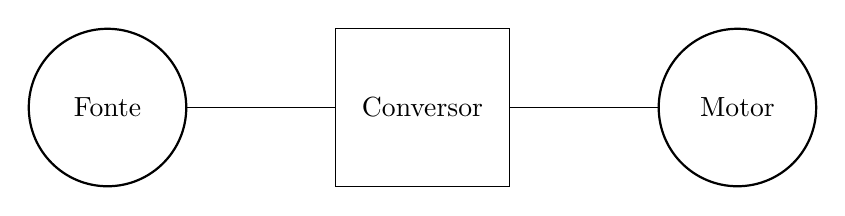
\begin{tikzpicture}
\node[circle,draw, minimum size = 2.0cm, thick](Fonte) at (0,0){Fonte};
\node[rectangle, draw, minimum width = 2.2cm, minimum height = 2.0cm](conv) at (4,0){Conversor};
\node[circle, draw, minimum size = 2.0cm, thick](motor) at (8,0){Motor};

\draw (Fonte) to[thick] (conv);
\draw (conv) to[thick] (motor);

\end{tikzpicture}
\caption{Sistema de conversão eletromecânica estudado.}
\label{fig:sistema}
\end{figure}

A fonte descrita na figura \ref{fig:sistema} pode representar o suprimento de energia em uma fábrica ou ambiente comercial em que o emprego do motor é necessário. Considera-se que ela fornece as tensões senoidais trifásicas e equilibradas, ou seja, tensões defasadas de 120º e com a mesma amplitude como nas equações a seguir.
\begin{align}
    V_a(t) &= V_M sin(\omega t) & [V] \\
    V_b(t) &= V_M sin(\omega t - 120^o) & [V] \\
    V_c(t) &= V_M sin(\omega t + 120^o) & [V] 
\end{align}

O motor do sistema funciona com a corrente alternada (CA) e pode ser aplicado em situações de velocidade variável, como, por exemplo, um veículo elétrico, em diversas máquinas na produção de papel,  máquinas da indústria têxtil, fabricação de cimento, linhas de produção de carros, etc. Tradicionalmente, as máquinas elétricas de CA foram usadas para aplicações com a frequência ou velocidade constante, enquanto as máquinas com corrente contínua (CC) foram preferidas para as aplicações com velocidades variáveis. Isso ocorreu devido à construção das máquinas CC que embora tenha desvantagens, como o maior custo por potência e problemas de manutenção com as escovas, possui um controle simples e a resposta do torque rápida. Por outro lado, as máquinas AC tem a construção mais robusta e um controle complexo. Essas questões motivaram muitas pesquisas sobre as aplicações de máquinas AC com a velocidade variável em conversores de potência \cite{Bose2}. Para o presente trabalho, o motor do sistema será o de indução. 
% Concertar essa figura.
\begin{figure}
    \centering
    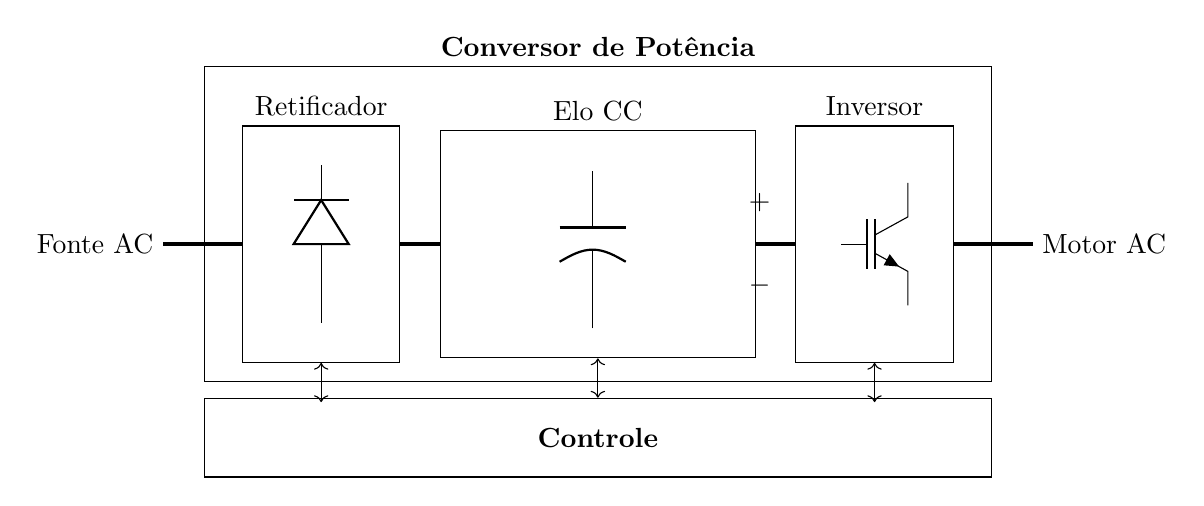
\begin{tikzpicture}[
	start chain = going right,
	box/.style = {
		on chain,join,draw,
		minimum height = 3cm,
		text centered,
		minimum width = 2cm,
	},
	every join/.style={ultra thick},
	node distance=5mm
]

\node [on chain] {Fonte AC}; % Chain starts here
\node [box, xshift=5mm, label = above: Retificador] (rec) {
	\begin{circuitikz}
		\draw (0,0) to[Do] (0,2);
	\end{circuitikz}
};

\node [on chain, join, draw, 
	text width=1cm,
	minimum width=4cm,
	minimum height=1.6cm,
	label=above:Elo CC,
] (ic) {
    \begin{circuitikz}[american voltages]
		\draw (0,0) to[pC, v<= $ $] (0,2);
	\end{circuitikz}
};

\node [box,label = above:Inversor] (inv) {
	\begin{circuitikz}
		\draw (0,0) node[nigbt] {};
	\end{circuitikz}
};

\node [on chain, join, xshift=5mm]{Motor AC};
% Chain ends here

% CU box
\node [
	rectangle,draw,
	below=5mm of ic,
	minimum width=10cm,
	minimum height=1cm,
] (cu) {\textbf{Controle}};

% PU box
\node [
	rectangle,draw,
	above=2mm of cu,
	minimum width=10cm,
	minimum height=4cm,
	label=\textbf{Conversor de Potência},
] (pu) {};

% Connections between CU and PU
\draw[<->] (rec.south) -- ++(0,-5mm);
\draw[<->] (cu.north) to (ic.south);
\draw[<->] (inv.south) -- ++(0,-5mm);

\end{tikzpicture}
    \caption{Diagrama de blocos com as diferentes partes de um conversor.}
    \label{fig:blocosdoconversor}
\end{figure}

O conversor conecta a fonte ao motor e, de uma forma geral, podemos descrever os seus componentes como a figura \ref{fig:blocosdoconversor}. A primeira etapa envolve a retificação do sinal através de uma "ponte" de diodo, figura \ref{fig:retificador}. Após a retificação, o elo CC, sustenta o nível de tensão através de um capacitor. Esse artifício torna o conversor alimentado por tensão, isto é, mantém-se a tensão para influenciar no sinal máximo a ser transmitido para o inversor. Por sua vez, o inversor funciona através da abertura e fechamento de chaves semi-condutoras na parte inversora e tem a corrente variável de acordo com as necessidades da carga. A topologia comum para o circuito trifásico pode ser vista na figura \ref{fig:inversor}.

\begin{figure}
    \centering
    \begin{circuitikz}
        % Pontos do circuitos
        \tkzDefPoints{ 0/2.5/A,
                       0/2.0/B,
                       0/1.5/C,
                       2/4/D,
                       2/2.5/E,
                       2/1.5/F,
                       2/0/G,
                       3.5/4/H,
                       3.5/2.5/I,
                       3.5/2.0/J,
                       3.5/1.5/K,
                       3.5/0/L,
                       5/4/M,
                       5/2.5/N,
                       5/1.5/O,
                       5/0/P,
                       6.5/4/Q,
                       6.5/0/R};
        % componentes
        \ctikzset{diodes/scale=0.6}
        \draw (E) to[D, l = D1] (D);
        \draw (G) to[D, l = D4] (F);
        \draw (L) to[D, l = D6] (K);
        \draw (I) to[D, l = D3] (H);
        \draw (P) to[D, l = D2] (O);
        \draw (N) to[D, l = D5] (M);
        \draw (R) to[C, v = $V_{CC}$] (Q);
        
        % conexões
        \draw (A) node[anchor = east]{A} to (E);
        \draw (E) -- (F);
        \draw (I) -- (J);
        \draw (J) -- (K);
        \draw (N) -- (O);
        \draw (B) node[anchor = east]{B} to (J);
        \draw (C) node[anchor = east]{C} to (O);
        \draw (D) -- (H);
        \draw (H) -- (M);
        \draw (M) -- (Q);
        \draw (G) -- (L);
        \draw (L) -- (P);
        \draw (P) -- (R);
        %\draw (
    \end{circuitikz}
    \caption{Topologia comum de uma ponte à diodo para retificação em um sistema trifásico.}
    \label{fig:retificador}
\end{figure}

\begin{figure}
    \centering
    \begin{circuitikz}[american]
    %% Definições dos pontos
    \tkzDefPoints{  0/0/A,
                    0/5/B,
                    2/5/C,
                    2/3/D,  %
                    2/0/E,
                    5/5/F,
                    5/2.5/G,%
                    5/0/H,
                    8/5/I,
                    8/2/J,  %
                    8/0/K,
                    2/4/t1,
                    2/1/t4,
                    5/4/t3,
                    5/1/t6,
                    8/4/t5,
                    8/1/t2,
                    11/2.5/M,
                    10/3/MA,
                    10/2.5/MB,
                    10/2/MC};
    %% componentes
    \draw (A) to[V, v=Vcc, invert] (B);
    \draw (t1) node[nigbt, bodydiode](T1){T1};
    \draw (t4) node[nigbt, bodydiode](T4){T4};
    \draw (t3) node[nigbt, bodydiode](T3){T3};
    \draw (t6) node[nigbt, bodydiode](T6){T6};
    \draw (t5) node[nigbt, bodydiode](T5){T5};
    \draw (t2) node[nigbt, bodydiode](T2){T2};
    \draw (M) node[elmech](M){M};
    
    %% ligações    
    \draw (B) -- (C);
    % leg A
    \draw (C) -- (T1.C);
    \draw (T1.E) -- (D);
    \draw (D) -- (T4.C);
    \draw (T4.E) -- (E);
    \draw (E) -- (A);
    % leg B
    \draw (F) -- (T3.C);
    \draw (T3.E) -- (G);
    \draw (G) -- (T6.C);
    \draw (T6.E) -- (H);
    \draw (H) -- (E);
    % leg C
    \draw (F) -- (I);
    \draw (I) -- (T5.C);
    \draw (T5.E) -- (J);
    \draw (J) -- (T2.C);
    \draw (T2.E) -- (K);
    \draw (C) -- (F);
    \draw (K) -- (H);
    % conectar ao motor
    \draw (D) -- (MA);
    \draw (MA) -- (M);
    \draw (G) -- (MB);
    \draw (MB) -- (M);
    \draw (J) -- (MC);
    \draw (MC) -- (M);
    
\end{circuitikz}
    \caption{Elo CC representado pela tensão $V_{CC}$ e a topologia comum de um inversor e suas conexões com o motor.}
    \label{fig:inversor}
\end{figure}

\subsection{O Papel da Proteção.}

A proteção para um \textit{drive} de velocidade variável, como descrito na sessão anterior, engloba os aspectos do próprio conversor e o motor associado. Para os \textit{drives} modernos, a maioria das funções de proteção são implementadas dentro do sistema de controle do conversor e com o foco na saída do sinal do conversor. Por isso, a proteção para a corrente na entrada (vinda da fonte) é comumente feita antes do conversor, próximo ao quadro de distribuição ou no centro de controle do motor, e inclui curto-circuito e faltas fase-terra. As principais funções de proteção que podem ser encontradas em um drive são \cite{BARNES2003}:

\begin{itemize}
    \item Subtensão CA na entrada do conversor;
    \item Subtensão CC no elo CC;
    \item Sobretensão CA na entrada do conversor;
    \item Sobretensão CC no elo CC;
    \item Sobrecorrente CA na saída do conversor;
    \item Falta fase-terra na saída do conversor;
    \item Altas temperatura no dissipador de calor;
    \item Sobrecarga térmica no motor.
\end{itemize}

As proteções contra subtensões tanto na entrada quanto no elo CC ocorrem apenas para certificar que o suprimento de energia está funcionando dentro das suas especificações, enquanto as proteções contra sobretensões e sobrecorrentes previnem os danos nos componentes do conversor. Assim como a sobrecorrente, as altas temperaturas, ocasionadas pelos ciclos de trabalho ou condições ambientais, limitam a vida útil dos semicondutores e a proteção garante que o sistema pare antes das faltas catastróficas, em que ocorre a destruição do equipamento.

A proteção contra faltas fase-terra é desenvolvida para detectar algum curto-circuito entre as fases e a terra. A sua função também é preservar o conversor e desconectar o equipamento assim que os limites são violados. Diferente das outras situações, a proteção fase-terra é usualmente implementada através de um transformador de corrente na saída do conversor. Esse dispositivo contém um núcleo toroidal magnético por onde as correntes passam e o secundário do transformador contém um circuito de baixa tensão que circula uma corrente caso a soma das correntes \( I_a\), \(I_b\) e \(I_c\) seja diferente de zero. 

A figura \ref{fig:protecaoConversor} ilustra as proteções citadas. Na entrada do conversor, os medidores calculam as tensões de linha \(V_{ab}\), \(V_{ac}\) e \(V_{bc}\) para a verificação de sobretensão e subtensão (SubT e SobT na figura); No elo CC, há medidores das tensões \(V_{CC}\) e correntes de linha \(I_{CC}\), para a verificação de sobretensão e sobrecorrente (CurtoC); Um sensor de temperatura verifica o estado das chaves semicondutoras (Temp).   
\begin{figure}
    \centering
    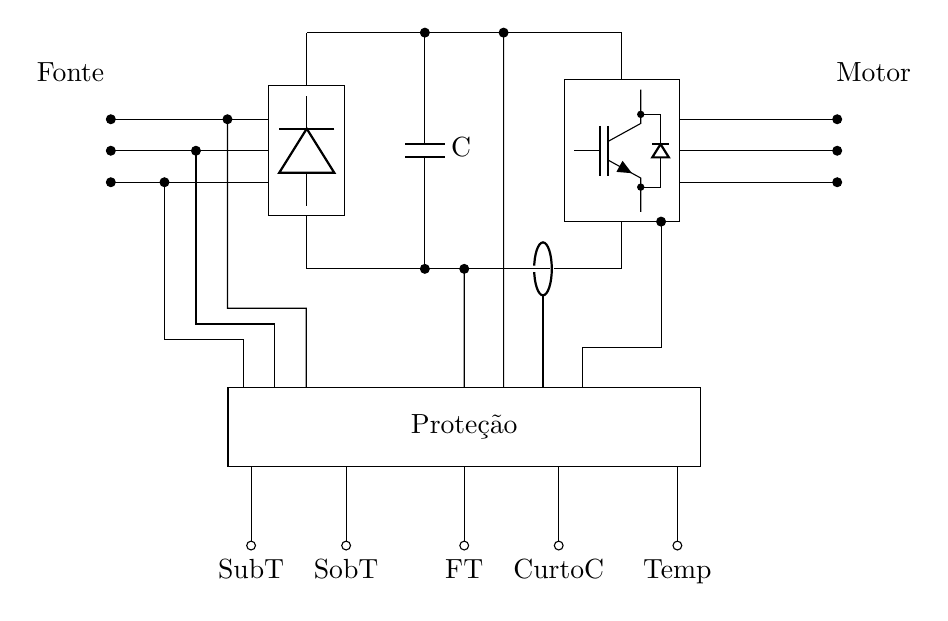
\begin{tikzpicture}
\tkzDefPoints{0/1/Ain,
              0/.5/Bin,
              0/0/Cin,
              2/1.5/A,
              3.5/1.5/B,
              4.5/1.5/C,
              6/1.5/D,
              2/-1.5/E,
              3.5/-1.5/F,
              5/-1.5/G,
              6/-1.5/H};

% retificador
\node [box,draw] at (2,0) (rec){
    \begin{circuitikz}
        \draw (0,0) to[D,scale = 0.7] (0,2);
    \end{circuitikz}
    };
    
% inversor    
\node [box, draw] at (6,0) (inv){
    \begin{circuitikz}
        \draw (0,0) node[nigbt, bodydiode]{};
    \end{circuitikz}
    };
    
\node [rectangle, draw,
       below = 15 mm of F,
       xshift = 5mm,
       minimum height = 1. cm,
       minimum width = 6 cm] (protec) {Proteção};

% conexões
\node[align = center] at (-1,1) {Fonte};
\node[align = center] at (9.2,1) {Motor};
\draw (rec.north) -- (A);
\draw (A) -- (B);
\draw (B) -- (D);
\draw (inv.north) --(D);
\draw (rec.south) -- (E);
\draw (E) -- (F);
\draw (F) -- ++(0.5,0);
\draw (F) ++(0.5,0) to[iloop, mirror, name = I] (H);
\draw (inv.south) -- (H);
\ctikzset{capacitors/scale=0.6};
\draw (B) to[C, l = C, *-*] (F);

\draw (rec.west) ++(0,0.4) to[short, -*] ++(-2,0);
\draw (rec.west) to [short, -*] ++(-2,0);
\draw (rec.west) ++(0,-0.4) to [short, -*] ++(-2,0);

\draw (inv.east) ++(0,0.4) to[short, -*] ++(2,0);
\draw (inv.east) to[short, -*] ++(2,0);
\draw (inv.east) ++(0,-0.4) to[short, -*] ++(2,0);

% conexões com o bloco da proteção.
\draw (protec.north) ++ (0.5,0) to [short, -*] (C);
\draw (F) ++ (0.5,0) to [short, *-] (protec.north) ++ (0.2,0);
\draw (protec.north) ++(1.5,0) to ++(0,0.5) to ++(1.,0) to [short,-*] ++(0,1.6);
\draw (protec.north) ++(1.,0) to (I.i);

\draw (protec.north west) ++(1.,0) to ++(0,1) to ++(-1.,0) to [short, -*] ++(0,2.4);
\draw (protec.north west) ++(.6,0) to ++(0,.8) to ++(-1.,0) to [short, -*] ++(0,2.2);
\draw (protec.north west) ++(.2,0) to ++(0,.6) to ++(-1.,0) to [short, -*] ++(0,2.);

% saída do bloco de proteção
\draw (protec.south west) ++(0.3,0) to ++(0,-1) node[ocirc, label = below:SubT]{};
\draw (protec.south) ++(-1.5,0) to ++(0,-1) node[ocirc, label = below: SobT]{};
\draw (protec.south) to ++(0,-1) node[ocirc, label = below: FT]{};
\draw (protec.south) ++(1.2,0) to ++(0,-1) node[ocirc, label = below: CurtoC]{};
\draw (protec.south east) ++(-0.3,0) to ++(0,-1) node[ocirc, label = below: Temp]{};
\end{tikzpicture}
    \caption{Esquema com as principais proteções para o conversor \cite{BARNES2003}.}
    \label{fig:protecaoConversor}
\end{figure}
% Incrementar com o livro do mamede e do coltrin.
% A diferença entre máquinas de grande porte e de pequeno porte.

\section{A Engenharia de Confiabilidade e a Eletrônica de Potência.}
% O que é
% Um pouco da história
% Subdivisões.
% Avanços.
A confiabilidade é a probabilidade de um item desenvolver a função exigida no tempo devido e em condições determinadas. Ela é frequentemente expressa pelo número de falhas em um período de tempo. Já a durabilidade é um aspecto da confiabilidade em relação a capacidade de resistir aos mecanismos dependentes do tempo, como a fadiga e a corrosão, e pode ser expressa em tempo mínimo antes da ocorrência de um desgaste, segundo \cite{Patrick2011_2}. A partir destas definições, esta seção se destina a entender um pouco do contexto histórico, as subdivisões e os avanços da área de engenharia de confiabilidade na eletrônica de potência.

\subsection{Contexto Histórico.}
O entendimento da engenharia de confiabilidade como uma disciplina foi possibilitado pelo desenvolvimento da estatística e o surgimento da produção em massa, isto é, a fabricação de bens de consumo em grandes quantidades \cite{SALEH2006249}, com o propósito de prevenir a criação de falhas o quanto antes possível, como na fase de \textit{design}. O motivo é que uma falha no \textit{design} tem efeito em todos os itens produzidos e o custo para a correção dos defeitos após a fabricação aumenta com a continuidade da produção. 

Uma das vertentes que predominou até os anos 80, sobretudo nos Estados Unidos, foram os métodos de previsão de confiabilidade quantitativa, ou seja, baseada em dados de falhas coletadas e publicadas em manuais providos pelo departamento de defesa norte-americano, como o MIL-HDBK-217F, e pela indústria. A principal premissa desses documentos era que a confiabilidade do sistema dependia dos componentes do sistema e precisava de dados de campo para os modelos estatísticos de previsão, que asseguravam taxas de falhas constantes \cite{Denson98}. 

As abordagens para a confiabilidade descritas no manual citado eram aceitáveis nos primórdios da eletrônica, quando as taxas de falhas eram altas e os circuitos menos complexos. Porém, com o avanço da tecnologia e a difusão de circuitos eletrônicos mais complexos, como os circuitos integrados, e de mais qualidade, cada vez mais evidências apontadas por especialistas da época sugeriam que o modelo de falha proposto pelo manual \cite{Denson98} não tinham precisão para prever as falhas e não eram atualizados para acompanhar o avanço tecnológico. Foi então que ocorreu uma mudança de entendimento gradual das causas das falhas dos sistemas em direção aos fatores ligados a sua aplicação, à fabricação, ao \textit{design}, às exigências do sistema, interface e software, que não foram computados nos modelos estatísticos antigos.

A partir desse cenário, uma outra abordagem para a confiabilidade com base nos processos físicos pelos quais as falhas ocorrem, chamada de \textit{Physics-of-failure} ou POF, passou a ter mais evidência. Há artigos de revisão como o de \cite{HuaiWang2021} que discorrem sobre essa mudança de paradigma em direção a POF, ou seja, da relevância da análise e a modelagem dos mecanismos de falha de um sistema contando com as cargas submetidas durante o seu uso e os aspectos ambientais em que esse sistema está submetido. Através desses modelos, pode-se descobrir os elos frágeis no produto para que as recomendações no design, produção, controle de processo, teste e operação em campo possam ser propostas.   

Por fim, através de uma linha temporal presente no trabalho de \cite{HuaiWang2021} e \cite{Chung2015}, figura \ref{fig:linhatemporal}, pode-se resumir os principais tópicos de pesquisas de cada época e fazer um paralelo entre a evolução da confiabilidade e da eletrônica de potência. A eletrônica de potência acompanhou o desenvolvimento das novas chaves semicondutoras, da possibilidade de produção e do controle e se beneficiou com os novos modelos para confiabilidade que surgiram no fim do século XX para suprir uma demanda da indústria e aplicações mais exigentes.

\begin{figure}
    \centering
    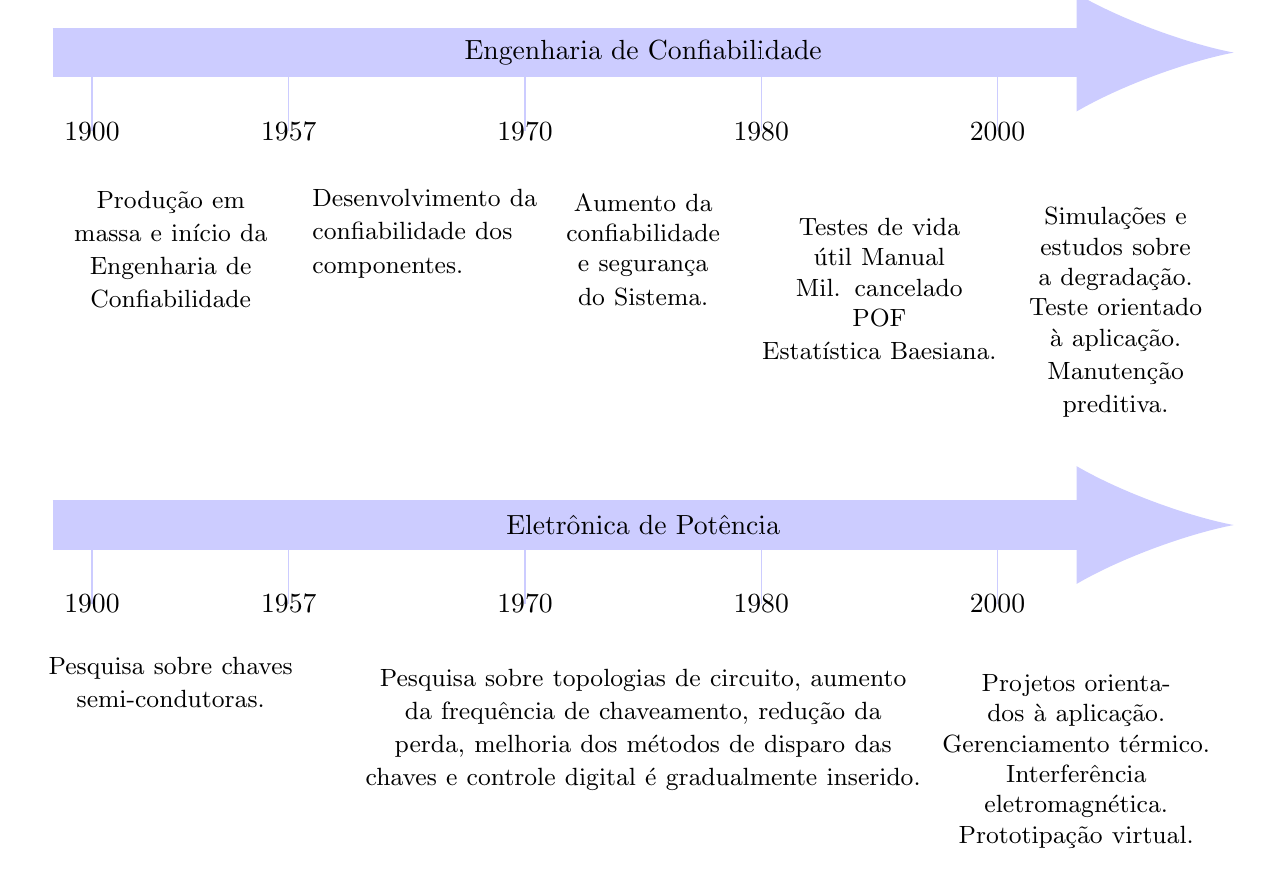
\begin{tikzpicture}
% textos da linha temporal da confiabilidade.
\node [align = center, text width = 3cm](texto1900) at (1.5, -2.5){\small Produção em massa e início da Engenharia de  Confiabilidade};
\node [align = left, text width = 3cm](texto1957) at (4.8, -2.3){ \small Desenvolvimento da confiabilidade dos componentes.};
\node [align = center, text width = 3cm](texto1970) at (7.5, -2.5){\small Aumento da confiabilidade e segurança \\\small do Sistema.};
\node [align = center, text width = 3.2cm](texto1980) at (10.5, -3.){\small Testes de vida útil Manual Mil. cancelado \\ \small POF\\ \small Estatística Baesiana.};
\node [align = center, text width = 3cm](texto2000) at (13.5, -3.3){\small Simulações e \\ \small estudos sobre a degradação. Teste orientado à aplicação.\\ \small Manutenção preditiva.};
%\draw[-{Triangle[width=18pt,length=8pt]}, line width=12pt](0,0) -- (15, 0);
\draw[->, >=latex, blue!20!white, line width=18pt] (0,0) to node[black]{Engenharia de Confiabilidade} (15,0);
\draw [blue!20!white](0.5,0.1) -- (0.5,-1.) node [black]{1900};
\draw [blue!20!white](3,0.1) -- (3,-1.) node [black]{1957};
\draw [blue!20!white](6,0.1) -- (6, -1.) node [black]{1970};
\draw [blue!20!white](9,0.1) -- (9, -1.) node [black]{1980};
\draw [blue!20!white](12,0.1) -- (12, -1) node [black]{2000};

% Textos da linha temporal de eletrônica de potência.
\node [align = center, text width = 3.2cm] at (1.5,-8){\small Pesquisa sobre chaves semi-condutoras.};
\node [align = center, text width = 7.2cm] at (7.5,-8.6){\small Pesquisa sobre topologias de circuito, aumento da frequência de chaveamento, redução da perda, melhoria dos métodos de disparo das chaves e controle digital é gradualmente inserido.};
\node [align = center, text width = 3.6cm] at (13,-9.0){\small Projetos orientados à aplicação. \\ \small Gerenciamento térmico. \\ \small Interferência eletromagnética. \\ \small Prototipação virtual. \\ };
\draw[->, >=latex, blue!20!white, line width=18pt] (0,-6) to node[black]{Eletrônica de Potência} (15,-6);
\draw [blue!20!white](0.5,-6.1) -- (0.5,-7.) node [black]{1900};
\draw [blue!20!white](3,-6.1) -- (3,-7.) node [black]{1957};
\draw [blue!20!white](6,-6.1) -- (6, -7.) node [black]{1970};
\draw [blue!20!white](9,-6.1) -- (9, -7.) node [black]{1980};
\draw [blue!20!white](12,-6.1) -- (12, -7) node [black]{2000};

\end{tikzpicture}

    \caption{Linha temporal de \cite{HuaiWang2021} e \cite{Chung2015} (adaptada) com os destaques da pesquisa da Eletrônica de Potência e da Engenharia de Confiabilidade por período de tempo no contexto desse trabalho.}
    \label{fig:linhatemporal}
\end{figure}

\subsection{A Pesquisa sobre a Confiabilidade em Eletrônica de Potência.}
Da perspectiva de \cite{Chung2015_2}, o futuro da pesquisa sobre confiabilidade em Eletrônica de Potência possui três pilares: A física analítica, design e verificação e controle e monitoramento. Esta seção descreve brevemente os conceitos desta perspectiva e ressalta o monitoramento das condições do conversor, a ênfase deste trabalho. 
\begin{figure}
    \centering
    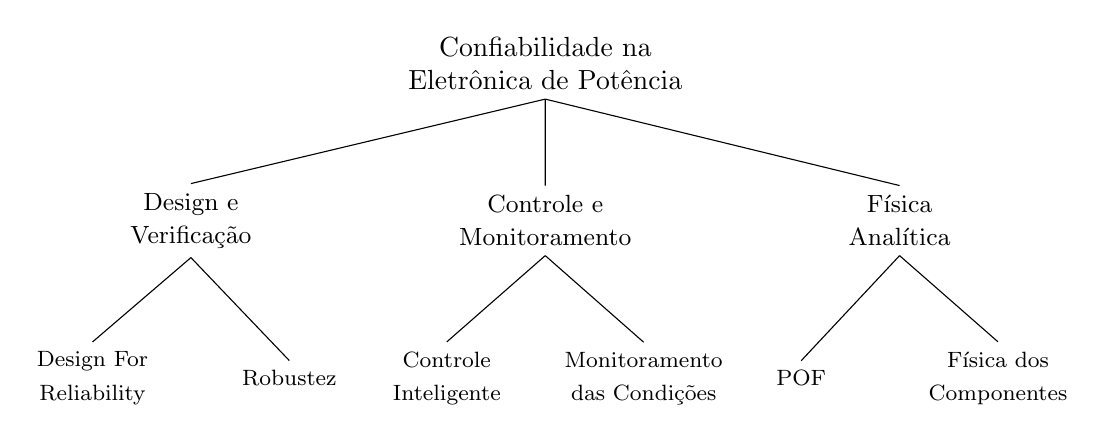
\begin{tikzpicture}
[
    level 1/.style = { sibling distance = 4.5cm},
    level 2/.style = { sibling distance = 2.5cm}
]
 
\node[align = center] {\normalsize Confiabilidade na\\\normalsize Eletrônica de Potência}[sibling distance = 2.cm, level distance = 2cm] 
    child [align = center]{node {\small Design e \\\small Verificação} child {node {\footnotesize Design For\\ \footnotesize Reliability}} 
    child {node {\footnotesize Robustez}}}
    child [align = center]{node {\small Controle e\\\small Monitoramento} child {node {\footnotesize Controle \\\footnotesize Inteligente}}
    child {node {\footnotesize Monitoramento \\\footnotesize das Condições}}}
    child [align = center]{node {\small Física\\\small Analítica}
    child {node {\footnotesize POF}}
    child {node {\footnotesize Física dos\\\footnotesize Componentes}}};
\end{tikzpicture}
    \caption{Os três pilares da pesquisa sobre Confiabilidade em Eletrônica de Potência.}
    \label{fig:pesquisaConfiabilidadeElePot}
\end{figure}

\subsubsection{Física Analítica}
O primeiro conceito necessário para uma eletrônica de potência mais confiável é entender a razão das falhas no nível do componente e dos sistemas através da sua análise física. A falha pode ocorrer de maneira súbita ou pela degradação no tempo. Pode-se entender a degradação do dispositivo no tempo através do esboço do gráfico da distribuição da capacidade do design (F) e das cargas (C) em que é submetido no ciclo de trabalho, como mostra a figura \ref{fig:degradacaonotempo}. O eixo x representa a carga (Por exemplo, temperatura, torque ou tensão) e o y, a frequência de aplicação de cada carga. Cada grandeza analisada pode ser alocada entre certos limites e representada por uma distribuição normal. Inicialmente, as cargas submetidas ao dispositivo estão respeitando os limites propostos pelo design a medida que nenhuma carga aplicada pode ser maior do que a capacidade do design. No entanto, a degradação atua de modo a enfraquecer o design por uma ação externa ou do próprio ciclo de trabalho até que uma parcela significativa da capacidade do design é afetada. Nesse ponto, determina-se o fim da vida útil do dispositivo. Isso implica que a falha pode ser adiada através de um aumento da capacidade do design ou pela aplicação da carga de forma reduzida com o tempo ou estado de degradação.   
\pgfmathdeclarefunction{gauss}{2}{%
  \pgfmathparse{1/(#2*sqrt(2*pi))*exp(-((x-#1)^2)/(2*#2^2))}%
}
\begin{figure}
    \centering
    
    \begin{tikzpicture}
\begin{axis}[
  no markers, domain=0:20, samples=100,
  axis lines*=left, xlabel=$x$, ylabel=$y$,
  every axis y label/.style={at=(current axis.above origin),anchor=south},
  every axis x label/.style={at=(current axis.right of origin),anchor=west},
  height=3.5cm, width=7.8cm,
  xtick={6,13.5}, ytick=\empty,
  enlargelimits=false, clip=false, axis on top,
  grid = major
  ]
  \addplot [very thick,cyan!50!black] {gauss(6,1)};
  \addplot [very thick,cyan!50!black] {gauss(13.5,1)};

\draw [yshift=-0.8cm, latex-latex](axis cs:10.5,0) -- node [fill=white] {F} (axis cs:16.5,0);
\draw [yshift=-0.8cm, latex-latex](axis cs:3.,0) -- node [fill=white] {C} (axis cs:9,0);

\end{axis}
\begin{axis}[yshift = 2.5cm, xshift = 1.79cm,
  no markers, domain=0:20, samples=100,
  axis lines*=left, xlabel=$x$, ylabel=$y$,
  every axis y label/.style={at=(current axis.above origin),anchor=south},
  every axis x label/.style={at=(current axis.right of origin),anchor=west},
  height=3.5cm, width=7.8cm,
  xtick={6,10.5}, ytick=\empty,
  enlargelimits=false, clip=false, axis on top,
  grid = major
  ]
    \addplot [fill=cyan!20, draw=none, domain=7.5:9] {gauss(6.,1)} \closedcycle;
  \addplot [very thick,cyan!50!black] {gauss(6,1)};
  \addplot [very thick,cyan!50!black] {gauss(10.5,1)};
  \end{axis}
  
  \begin{axis}[yshift = 5.cm, xshift = 3.5cm,
  no markers, domain=0:20, samples=100,
  axis lines*=left, xlabel=$x$, ylabel=$y$,
  every axis y label/.style={at=(current axis.above origin),anchor=south},
  every axis x label/.style={at=(current axis.right of origin),anchor=west},
  height=3.5cm, width=7.8cm,
  xtick={6,9.7}, ytick=\empty,
  enlargelimits=false, clip=false, axis on top,
  grid = major
  ]
  \addplot [fill=cyan!20, draw=none, domain=6.6:9] {gauss(6.,1)} \closedcycle;
  \addplot [very thick,cyan!50!black] {gauss(6,1)};
  \addplot [very thick,cyan!50!black] {gauss(9.7,1)};
  \addplot [very thick,magenta!30!white, dash pattern = on 3pt off 3pt] {gauss(13.5,1)};
  \end{axis}
  \draw [->](0,0) -- (55:7.cm);
  \draw (0,0) -- (55:3.5cm)node [ midway, above, sloped, align = center] (TextNode) {\small tempo};
  \draw [magenta!30!white,dash pattern=on 3pt off 3pt](3.3,0) -- +(55:6cm);
  \draw [magenta!30!white,dash pattern=on 3pt off 3pt](5.,0) -- +(55:6cm);
  \node [align = center](texto) at (8.6,3.5){Falta};
  \draw [->, thick, cyan!80!white, bend left = 20](texto.west) to +(155:2.3cm);
  \node [align = center](textoprojecao) at (8.8,7){Projeção};
  
\end{tikzpicture}
    \caption{Figura com a explicação para a falha através do tempo de serviço de \cite{Chung2015_2}. A legenda 'C' representa a carga do disposito e 'F' representa a força ´máxima suportável por design.}
    \label{fig:degradacaonotempo}
\end{figure}
% POF
\subsubsection{Design e Verificação}

\subsubsection{Controle e Monitoramento}
% Controle Inteligente
\subsection{O Monitoramento das Condições de um Conversor.}

\section{A Detecção de Faltas.}
\subsection{As faltas do ponto de vista dos IGBTs.}
\subsection{As faltas do ponto de vista do conversor.}
\subsection{As faltas do ponto de vista da fonte.}
\subsection{As faltas do ponto de vista do elo CC.}
\subsection{As faltas do ponto de vista do motor de indução.}

\section{Revisão Sobre a Detecção de Faltas de CA.}
\subsection{Os Caminhos de Detecção Através do Hardware.}
\subsection{Os Caminhos de Detecção Através do Software.}
\section{Resumo do Capítulo.}

%%%%%%%%%%%%%%%%%%%%%%%%%%%%%%%%%%%%%%%%%%%%%%%%%%%%%%%%%%
\chapter{Métodos}
\section{A Simulação}
Esse trabalho desenvolve um estudo sobre a detecção de faltas em um conversor controlador de um motor de indução trifásico. O estudo será por meio de simulação no ambiente do Simulink, através da biblioteca de \textit{Specialized Technology} dentro do d
\subsection{A configuração da proteção}
\subsection{O motor}
\subsection{O controle}
\subsection{Elo CC}


\section{O método para detecção de faltas}

\section{A determinação do estado normal e estado anormal de atuação.}

\section{Os casos estudados}

\chapter{Resultados e Discussões}
\section{Análise dos sinais de corrente nos casos estudados.}

\subsection{Possíveis efeitos no motor de Indução.}

\section{Detecção de faltas nas chaves semicondutoras.}

\subsection{Faltas do tipo circuito aberto.}

\subsection{Faltas de caráter intermitente no disparo drive.}

\section{Resumo do método proposto e seus resultados.}

%%%%%%%%%%%%%%%%%%%%%%%%%%%%%%%%%%%%%%%%%%%%%%%%%%%%%%%%%%
\chapter{Conclusões}

\backmatter
\bibliographystyle{coppe-unsrt}
\bibliography{Bibliografia}

\appendix
\chapter{Algumas Demonstra{\c c}\~oes}
\end{document}

